\documentclass[11pt,a4paper]{report}

% Aberstwyth dissertation LaTeX Template
% Authors: Dr. Hannah Dee (hmd1@aber.ac.uk), Neil Taylor (nst@aber.ac.uk)
% This has been adapted from the Leeds Thesis template and the 
% Group Project template for Computer Science in Aberystywth University.
% 
% All comments and suggestions welcome.
%
% Template designed to be used with pdflatex: it may need alteration to
% run with a different LaTeX engine

% To build document on the unix command line, run four commands:
 
% pdflatex dissertation
% bibtex dissertation
% pdflatex dissertation
% pdflatex dissertation

% you will end up with dissertation.pdf 
\usepackage{mmp}

% the following packages are used for citations - You only need to include one. 
%
% Use the cite package if you are using the numeric style (e.g. IEEEannot). 
% Use the natbib package if you are using the author-date style (e.g. authordate2annot). 
% Only use one of these and comment out the other one. 
%\usepackage{cite}
\usepackage{natbib}

% Use the following to selectively exclude chapters
%\includeonly{cover,abstract,acknowledge,declare,chapter1,chapter2}

\begin{document}

% all of the include directives below refer to tex files
% so 
\title{Kyffin Williams: Digital Analysis of Paintings}

% Your name
\author{Alexander David Brown}

% Your email 
\authoremail{adb9@aber.ac.uk}

\degreeschemecode{G601} %e.g. G400 
\degreeschemetitle{Software Engineering} % e.g. Computer Science
\degreetype{Master of Engineering}

\modulecode{CS39440} % i.e. CS39440, CC39440, CS39620
\moduletitle{Major Project} % i.e. Major Project or Minor Project

\date{22nd April 2012} % i.e. the date of this version of the report

\status{Release} % Use draft until you create the release version. Then, change this to Release.
\mmpversion{1.0.0}

%The title and name of your supervisor.
\supervisor{Hannah M. Dee} 

%The email for your supervisor. 
\supervisoremail{hmd1@aber.ac.uk}

\maketitle



 includes cover.tex - to change the content,
% edit the tex file

\pagenumbering{roman}

% This is the front page

\title{Kyffin Williams: Digital Analysis of Paintings}

% Your name
\author{Alexander David Brown}

% Your email 
\authoremail{adb9@aber.ac.uk}

\degreeschemecode{G601} %e.g. G400 
\degreeschemetitle{Software Engineering} % e.g. Computer Science
\degreetype{Master of Engineering}

\modulecode{CS39440} % i.e. CS39440, CC39440, CS39620
\moduletitle{Major Project} % i.e. Major Project or Minor Project

\date{22nd April 2012} % i.e. the date of this version of the report

\status{Release} % Use draft until you create the release version. Then, change this to Release.
\mmpversion{1.0.0}

%The title and name of your supervisor.
\supervisor{Hannah M. Dee} 

%The email for your supervisor. 
\supervisoremail{hmd1@aber.ac.uk}

\maketitle



                        

% Set up page numbering
\pagestyle{empty}

% declarations of originality 
\thispagestyle{empty}

%%%
%%% You must sign the declaration of originality. 
%%%
\begin{center}
    {\LARGE\bf Declaration of originality}
\end{center}

In signing below, I confirm that:

\begin{itemize}
\item{This submission is my own work, except where clearly
indicated.  }

\item{I understand that there are severe penalties for plagiarism 
and other unfair practice, which can lead to loss of marks
or even the withholding of a degree. }
 
\item{I have read the sections on unfair practice in the Students' 
Examinations Handbook and the relevant sections of the 
current Student Handbook of the Department of Computer 
Science.}
 
\item{I understand and agree to abide by the University's
regulations governing these issues.}
\end{itemize}

\vspace{3em}
Signature ............................................................  \\

\vspace{1em}
Date ............................................................ \\

%%% 
%%% We would like to make a selection of final reports available to students that take 
%%% this module in future years. To enable us to do this, we require your consent. You 
%%% are not required that you do this, but if you do give your consent, then we will have 
%%% the option to select yours as one of a number of reports as examples for other 
%%% students. If you would like to give your consent, then please include the following 
%%% text and sign below. If you do not wish to give your consent, please remove this 
%%% from your report. 
%%%
\vspace{5em}
\begin{center}
    {\LARGE\bf Consent to share this work}
\end{center}

In signing below, I hereby agree to this dissertation being made available to other
students and academic staff of the Aberystwyth Computer Science Department.  

\vspace{3em}
Signature ............................................................  \\

\vspace{1em}
Date ............................................................ \\

               

\thispagestyle{empty}

\begin{center}
    {\LARGE\bf Acknowledgements}
\end{center}

%To Llyod, Hannah and the Cooper's Arms for setting the scene for this crazy project.

%To Jade, Kate, Yarrow and Sam for being great friends in times of need.

%To Kyffin Williams himself, for being such an interesting artist.

%To the writers of the neumerous libaraies I have used in this project, without which I would have been stumped at day one.

%Finally, though she already been mentioned, to Hannah who has been everything a student could want in a supervisor and a lot more. For the crazy ideas and piles of reading material. And for getting me to cite Rolf Harris.
 % Acknowledgements
\thispagestyle{empty}

\begin{center}
    {\LARGE\bf Abstract}
\end{center}

%Include an abstract for your project. This should be no more than 300 words.
Sir John ``Kyffin'' Williams was a Welsh landscape painter widely regarded as the defining artist of Wales during the 20\textsuperscript{th} century.

%FIXME Find out the name of the art historian at NLW.
???, an Art Historian working with the National Library of Wales has collected a lot of information about Kyffin Williams' paintings; including, where known, the date the painting was created (or a range of years where the exact year is not know) and the location depicted by the painting. 

This information allows for some interesting analysis to be performed on Kyffin Williams' paintings: temporal analysis to classify the date of paintings for which the actual date is unknown or to narrow down the range of dates; or geographical analysis to be able to classify the location the painting depicts.

Of the two, temporal anaysis is the more viable; geographical analysis would have to assume the scene was painted fairly exactly. Most artists take liberties with the details of the subject making it even more difficult to accurately location the painted location. Temporal analysis can potentially be more concrete as changes in style are likely to be less extreme than the liberties taken with the details of a subject.


                 % Abstract

\pagenumbering{roman}
\pagestyle{fancy}
\fancyhead{}
\fancyfoot[C]{\thepage}
\renewcommand{\headrulewidth}{0 pt}
\renewcommand{\chaptermark}[1]{\markboth{#1}{}}

\tableofcontents   
\newpage
\listoffigures
\newpage 
\listoftables
\newpage

% Set up page numbering
\pagenumbering{arabic}

\setchapterheaderfooter

% include the chapters
\chapter{Background \& Objectives}

%This section should pick-up material from your progress report and enhance it based on the feedback and also your additional experience up to now. 

\section{Sir John ``Kyffin'' Williams}

Sir John ``Kyffin'' Williams (1918-2006) was a Welsh painter and printmaker, widely regarded as 
the defining artist of Wales during the 20\textsuperscript{th} century\cite{Davies2008Welsh}. He was advised to take up
art by a doctor after failing a British Army medical examination because of an `abnormality' 
(epilepsy) as something which would not tax his brain.

He studied at the Slade School of Fine Art and taught art in Highgate School, after which he 
retired to Anglesey until he died in 2006 after a long battle with cancer.

His most characteristic pictures are of Welsh landscapes, painted with thick layers of oil paint
applied with a palette knife\cite{Chilvers2009Dictionary}. Most of his paintings are highly textural; to the point of being
3-dimensional.

As his life progressed Kyffin's `abnormality' grew steadily worse, especially when exposed to 
bright light. As a result most of his paintings are of overcast Welsh landscapes and tend to 
become visibly darker over time\cite{Harris2011How}. By eye it is generally quite easy to approximate the time period
in which a painting was created.

In 1969 he won a scholarship to study and paint in Y Wladfa; the Welsh settlement in Patagonia.
This period of his life is very obvious from his paintings as there is a complete contrast in 
colour between Patagonian and Welsh landscapes.


\section{Interdisciplinary work with the National Library of Wales}

% FIXME Llyod's Thesis Title
This project was initially suggested through a conversation between Hannah Dee and Gareth ``Llyod''
Roderick about image processing and art. Llyod is a PhD student at the \gls{nlw}.
Their initial idea was to try to geolocate a Kyffin painting on a map to build up a geographical 
representation of Kyffin's work.

Hannah started to create a prototype for performing geographical analysis, this proved to be a 
difficult task and one which is still being researched.

However, the nature of Kyffin's illness and painting style allows for a second form of analysis:
temporal. As previously stated it is fairly easy to judge by eye a good approximation of the 
period in which a Kyffin painting was created. It should, therefore, follow that this process can
be performed digitally.

When I started this project I was given a ``database'' (in reality this was just a spreadsheet) 
Llyod had produced, containing information of Kyffin Williams' paintings, including: title, year,
category (landscape, portrait, etc.), canvas size and a few additional details which aren't so 
relevant to the project.

The first meeting held was between Llyod, Hannah and I, in which we discussed the current state of
the project, what our aims for the project were and what form of help Llyod could provide to us.
As one of the objectives of this project is to, eventually, get a paper published, the relevant
details of the process we would need to go through if we wanted to do so.

The second meeting was between Hannah, Llyod, Lorna M. Hughes (Llyod's supervisor) and I. Again we
discussed the state of the project. Llyod had also produced a better version of his ``database'' 
to be more machine readable and succinct. A lot of information came from this meeting;

\begin{itemize}
\item The ``cut-off'' point between early and late is around 1973.
\item The size of the canvas might be a useful data point to use in classification, as Kyffin sold
more paintings he would have had the money available for larger canvases and the paint for said
canvas.
\item It is a little dubious as to whether some dates can be trusted. One painting owned by the
NLW was stated to be his last painting, but Lorna believes it was painted much earlier and claimed
to be his last to improve the sale price.
\item Llyod may have found date markings on some paintings. These again may not be accurate, but
may prove to increase the sample size.
\item It should be easy to provide a ``no later than'' estimate for each painting from the art
historians.
\item Paul (?) should be able to produce some exemplars for us as a ground truth.
\item Llyod may be able to find more paintings in the hands of private collectors to increase the 
sample size.
\item Llyod had been playing around with ImageJ to do some basic graph plotting. This might be 
useful to look at further to expand my own work.
\end{itemize}

There were also more detailed discussions about publications, particularly in a digital humanities
journal.


\subsection{Continuation of the Kyffin Project}

There are several projects that could continue on from the Kyffin Project.

One was to use the Learning/Teaching development fund to produce a web-based front-end for of some
of my analysis.

Another venture was to look into PhD funding to build up a 3D map of some of Kyffin's paintings
and being able to display it (perhaps via HTML5 and WebGL) so they can explore the painting 
digitally how it is meant to be in real life.



\section{Existing Work}

\subsection{Edge-Orientated Gradients}\label{sec:existing-hogs}

\subsection{Brush-stroke Analysis}\label{sec:existing-brush-stroke}
Stroke analysis is one of the main goals for this project. It is quite apparent from looking at 
Kyffin Williams' paintings that his brush-strokes change over time, his early work having lots of
smaller strokes over the canvas to large bold strokes in his later work.

The first paper I found relating to the analysis of brush-strokes involved moving a circular filter
across the whole painting to find the ridges of strokes, then filling any unbroken areas. They then
shrunk these areas to a single pixel line and fitted a $n^{\text{th}}$ order polynomial to this
line\cite{Berezhnoy2005Authentic}. This method seems fairly simplistic, but could be an interesting
first step, but as it is more focused on authenticating paintings it may be of limited use.

Another method for stroke analysis has been published in the IEEE Transactions on Pattern Analysis
and Machine Learning journal. This method is far more complex, but is able to extract and label
individual brush-strokes. An interesting part of their findings was the ability to date some of Van
Gogh's paintings to a known period in his career\cite{Li2012Rhythmic}.

This method involves performing edge detection of the painting followed by an edge linking 
algorithm which aims to remove small, noisy edges and to trace every edge. With this they then
perform enclosing, as strokes may not be complete this stage also aims to fill in missing gaps of
strokes and to fill these in within a certain tolerance.

The algorithm then decides if a stroke really is a painted stroke, if the stroke is completely 
enclosed, isolated from other non-edge pixels and forms a connected component then it is likely 
that it is a proper brush-stroke and is extracted. The edge pixels are used as the background and
the non-edge pixels as the foreground, this is the process of labelling the brush-stroke.

For each of these labelled candidates, a heuristic function is used to threshold any brush-strokes 
that are either too long or too short, these strokes are discarded. These strokes are then
considered to be candidates if they are not significantly branched, the stroke is not too wide 
(this may change for Kyffin Williams as he used a pallet knife rather than a brush) and the 
brush-stroke is not too big or small.

Separately, the image is then segmented using $k$-means clustering by \gls{rgb} values. This clustering 
algorithm is applied several times, lowering the tolerances for distance within a cluster. 
Connected components as a result of this clustering and have noise reduction performed upon them.
Finally, the two types of brush-strokes are combined.

This technique may need some changing to account for Kyffin Williams' use of a pallet knife, but
the overall principals of this technique should work with Kyffin's paintings.


\section{Analysis Objectives}
Analysis is one of the biggest sections of this project and involves creating techniques which 
will allow comparison of paintings in a way which will allow some form of classification to be
performed on them.

Typically I would expect this to produce some form of high-dimension state space in which each
painting is a point in the state space. From this state space the distance between one painting
and another can be easily resolved using a distance measure like Manhattan distance 
\eqref{eq:manhattan_distance}, euclidean distance \eqref{eq:euclidean_distance} or a distance 
measure more specific to the state space should it be needed (e.g.: chi-squared for histograms).

\begin{equation}\label{eq:manhattan_distance}
d_1(\mathbf{p},\mathbf{q}) = \|\mathbf{p}-\mathbf{q}\|_1 = \sum^{n}_{i=0}{|p_i-q_i|}
\end{equation}

\begin{equation}\label{eq:euclidean_distance}
d_1(\mathbf{p}, \mathbf{q}) = \sqrt{\sum^{n}_{i=0}({q_i-p_i})^2}
\end{equation}

\subsection{Colour-space Analysis}
The simplest way of analysing a digital image is to look at the colours which it consists of.
Doing this is relatively simple; each pixel has a set of values defining the colour of that point,
getting something meaningful from this is less simple.

The simplest strategy is to perform some form of statistical analysis on each painting then use
this for classification. Several good and computationally cheap options exist for this; 
mean \eqref{eq:mean} and standard deviation \eqref{eq:std_dev}, are some good
examples which often come predefined in image processing and computer vision libraries.

\begin{equation}\label{eq:mean}
\upmu = \frac{1}{N}\sum_{i=1}^{N}x_i
\end{equation}

\begin{equation}\label{eq:std_dev}
\sigma = \sqrt{\frac{1}{N}\sum_{i=1}^{N}(x_i - \upmu)^2}
\end{equation}

The representation of colour is another important factor, an \gls{rgb} representation will have all 
three values change if there are many changes in brightness of the colours whilst a \gls{hsv} 
representation will only have a single value change.

Therefore, an object of this section should be to explore different colour models and statistical
methods which can be applied to them.

Another useful technique which should be investigated early into the project are image histograms.
These histograms plot the distribution of colour across an image and are therefore a very powerful
method of analysing an image, especially for comparison. As with statistical analysis, histograms
will be largely effective by colour model.

\subsection{Texture Analysis}
As Kyffin Williams' work is very textural, it follows that a main part of the analysis should
focus around the texture of his paintings. Unfortunately for this section, it seems unlikely that
I will be able to get any 3-dimensional models of Kyffin's paintings. This would have been a nice,
if rather large, section of the project.

Instead it is more sensible to look at the orientation of edges in Kyffin's work. Some useful 
pre-existing techniques have already been discussed in section~\ref{sec:existing-hogs}. Histograms
of edge orientation\cite{Dalal2005Histograms} seem like a promising concept which may prove 
relatively simple to implement.

This section may also help with any work into brush-stroke analysis (see 
section~\ref{sec:analysis-brush-stroke}).

\subsection{Brush-stroke Analysis}\label{sec:analysis-brush-stroke}
With Kyffin's distinctive style and how obviously this style changes over time, the ultimate aim 
of this project is to be able to analyse the brush-strokes\footnote{A slight misnomer as Kyffin 
used a palette knife to paint with rather than a traditional brush} in a painting.

From looking at the paintings it is very apparent that in his earlier work he made a lot more 
strokes than in his later works\footnote{Although this isn't quite true as the canvases he worked
on in his later life tended to be larger}. The strokes in his later work tend to have larger areas
and span more of the canvas.

If it is possible to calculate a rough amount and size of strokes made in a given painting it 
should be a reasonable piece of data to classify on. As previously discussed in section~
\ref{sec:existing-brush-stroke} there has already been a decent amount of research into determining
brush-strokes in a painting. 

It would be preferable to try and take one of the techniques discussed in that research and change
it to suit the needs of the project rather than attempting to create a whole new method of 
brush-stroke recognition.

\subsection{Ensemble Techniques}
With some of the aforementioned analysis techniques it makes sense to combine two or more 
techniques together; a good example would be colour histograms and histograms of edge orientation.

This form of analysis is inspired by the concept of the same name in statistics and machine 
learning which tend to obtain better predictive performance. It may also be worth while trying to
weight different techniques so that the techniques which give the best performance affect the 
result of the ensemble technique more.


\section{Classification Objectives}
The overall objective of classification is to be able to label a painting by Kyffin Williams as 
being painted in a given year based on analysis performed on all other paintings with known years.

This ties in with the main aim of this project of being able to classify any Kyffin Williams
painting, whether it has a known or unknown year, as being from a given year. Evidently for 
paintings with an unknown year it is difficult to know how accurately the system has been, so, for
the most part, these paintings have been ignored and those paintings with a known year have made
up the training and validation set.

Because of the small size of paintings with known years it should be computationally viable to 
perform leave-one-out cross validation (figure~\ref{fig:loocv}).

\begin{figure}[h]
\begin{algorithmic}
\Function{LOOCV}{$data$} \Comment{$data$ is a set of all data points}
  \ForAll{$item \in data$}
    \State $classified_{item} \gets$ \Call{Classify}{$item, data \setminus \left\{{item}\right\}$} 
  \EndFor
  \Statex
  \Return $classified$
\EndFunction
\end{algorithmic}
\caption{Pseudocode for Leave-One-Out Cross Validation}\label{fig:loocv}
\end{figure}

This can be used to evaluate the performance of the analysis technique and classification 
algorithm. Pearson's product-moment correlation coefficient \eqref{eq:pearsons} between actual year
and classified year has been suggested to be a good performance measure for this project.

\begin{equation}\label{eq:pearsons}
\rho_{X,Y}={\mathrm{cov}(X,Y) \over \sigma_X \sigma_Y} ={E[(X-\mu_X)(Y-\mu_Y)] \over \sigma_X\sigma_Y}
\end{equation}


\subsection{Classification}
One of the simplest methods of classification is $k$-Nearest Neighbour (figure~\ref{fig:knn}) from
this one can take a poll of the years for each neighbour and assign the year of the painting to
classify to be the average of these years.

Depending which form of average you take (mathematical mean \eqref{eq:mean}, median or mode) will
alter the result; although it should be noted that median is very unlikely to give a result on its
own due to the sparseness of the data.

\begin{figure}[h]
\begin{algorithmic}
\Require{$0 < k \leq \left|{data}\right|$} \Comment{$data$ is a set of all data points}
\Function{KNearestNeighbour}{$k, data$}
  \For{$i = 1 \to k$}
    \State $nn_i \gets \Call{Nearest}{data}$
    \State $data \gets data \setminus \left\{{nn_i}\right\}$
    \State $i = i + 1$
  \EndFor
  \Statex
  \Return $nn$
\EndFunction
\end{algorithmic}
\caption{Pseudocode for $k$-Nearest Neighbour}\label{fig:knn}
\end{figure}

There are other techniques which could be applied to this problem, but the rewards for 
implementing them is not likely to be outweighed by the time it would take to implement such
techniques. There is a workaround for this; there are several machine learning tool-kits which 
provide pre-implemented version of these techniques.

One of the most popular tool-kits available for general use is Weka\cite{Hall2009WEKA}, which is discussed in more
detail in section~\ref{sec:bg-weka}.

% FIXME Find out who Julie is here.
Another technique suggested by Julie Greensmith is to use \gls{lcs}\cite{Bacardit2013Largescale}, 
which has an implementation for Weka. This may prove to give very good results for the kind of
analysis being performed on Kyffin's work.

\subsubsection{Use of Weka}\label{sec:bg-weka}

%\subsubsection{Learning Classifier Systems (LCS)}

\subsection{Exemplars}
The use of exemplar images would be another way of performing classification. The idea of an 
exemplar is that a painting is the most representative of a given time period. With the help of
Llyod, Lorna and the \gls{nlw} a list of exemplars which can be used as a ground truth to classify
against has been produced.

The initial idea for digitally producing exemplars is to take the middle painting for a time 
period, as would be expected. These can then be compared to the ground truths to see how correct
the analysis technique performed.

However, there is also the potentially to generate a theoretical exemplar from the analysis. This
might be hard to perform validation against the ground truth upon, but will give some useful data
on Kyffin Williams' style and how it changed.

These theoretical exemplars would likely be produced using some form of Gaussian mixture model.

%\addcontentsline{toc}{chapter}{Development Process}
\chapter{Development Process}

%You need to describe briefly the life cycle model that you used. Do not force your project into the waterfall model if it is better described by prototyping or some other evolutionary model. You do not need to write about all of the different process models that you are aware of. Focus on the process model that you have used. It is possible that you needed to adapt an existing process model to suit your project; clearly identify what you used and how you adapted it for your needs.

%In most cases, the agreed objectives or requirements will be the result of a compromise between what would ideally have been produced and what was felt to be possible in the time available. A discussion of the process of arriving at the final list is usually appropriate.

%You should briefly describe the design method you used and any support tools that you used. You should discuss your choice of implementation tools - programming language, compilers, database management system, program development environment, etc.

This chapter defines the development processes which were used to write this project and how they
were changed to suit the needs of this project. The decisions behind the choices
of development process are also discussed and evaluated.

\section{Introduction}
This project was developed using a mixture of iterative development and rapid prototyping. As a
research project it does not need a heavy-weight development process as such a process would be
too cumbersome to adapt to changing nature of research. Agile methodologies would have also 
provided the adaptability required, but are designed for a team-based approach so would have
needed a lot of modification to be applicable to a team of one.

Maintenance and testing are known to be the large majority of focus in the methodology chosen,
experience in the field of software engineering typically focuses an individual on both these 
topics. However as this was a research project it was unlikely to be used much after the end of 
the project and if it was to be the author or the supervisor would be able to provide to anyone
using or extending the project. It was decided that maintenance was not an issue for this project
and could be, to a reasonable extent, ignored.

Due to the research nature of this project testing would prove to be difficult. Proving that a
given technique would run was relatively straight-forward by leaning on the interpreter (or 
compiler in cases of any statically typed elements), but proving a technique would do what it was
expected to do would take so much time out of implementing other techniques that it would be a 
pointless task, especially when a lot of the techniques would just call external libraries to
implement the parts that were likely to fail (e.g. applying filters through \gls{opencv}).

With both these two issues being lesser than usual it was easy to remove a lot of the traditional
and formal methods from the list of potential methodologies; Waterfall and Spiral models, for 
example, had too much of a focus on both these parts and on risk management.

Iterative development involves developing a system through repeated cycles, at each iteration 
design modifications are made and new functionality is added. Iterative development encourages 
modular design and implementation, suiting this project well as it will have a number of 
techniques to both analyse and classify data points.

Rapid Prototyping involves quickly producing a working prototype of an area of a system to get a
working implementation of that area. This can then be evolved to improve the design and 
implementation as needed. This fits well as a method for implementing the various techniques in 
the system, they can be rapidly prototyped to get a set of results, then improved to increase the
performance and/or accuracy of the technique.

The requirements for the iterations were typically decided in the weekly project meetings, typically 
taking the form of completing a given technique before the next meeting. The technique
was then implemented as a prototype and any adjustments would be made to the system in line with
the iterative process, including improving existing techniques that might have been earlier 
prototyped in an evolutionary fashion.

Initially there were a set of topics which were aimed to be completed:

\begin{itemize}
\item Colour-space analysis
\item $k$-Nearest Neighbour classification
\item Histogram-based colour-space analysis
\item Texture analysis
\item Brush-stroke analysis
\end{itemize}

Each of the above items had several parts to them; colour-space analysis included different 
colour-modes: \gls{rgb} and \gls{hsv}. However as a research project new ideas were often 
suggested during meetings or as a part of research so this list of requirements grew during the
project.

Python helped a lot with both methodologies, thanks to it's dynamic typing it is easy to deal with
changing forms of data. It also has very readable syntax whilst still remaining compact in terms
of lines of code, this makes locating areas which need changing very simple.

Version control was a strong requirement. Having used git for many personal projects the 
environment was familiar, the decentralised nature of git allowed for the remote working on any
machine with an internet connect so progress was not delayed with the switching of computers.

For hosting the GitHub service was used, GitHub is one of the most popular git hosting services
available and offers free private repositories for students (GitHub is commonly used for Open 
Source software development so most repositories are public by default). It should be noted that
this service is known to be very stable and reliable, but even during brief moments of downtime,
the decentralised nature of git meant that work could continue regardless.

\section{Modifications}
%Did you have to modify the model to suit a one-person project. If so, what did you change and why? 

The main modifications made to iterative development was to shift focus away from testing and into
evolution and implementation. It was also changed to that each iteration was a rapid prototype,
to allow merging of the two techniques. But the evolution step was focused on the whole system.
A good example of this is when finding out about \emph{cv2} and going back to change all the old
techniques to use the latest version of \emph{OpenCV}.

Rapid prototyping was modified very little, however, as there was no official client and only met with
Hannah once a week there was very little client focus and was just used as a tool for rapidly
implementing techniques in a way which could be improved and evolved later on. Although this isn't
exactly in the spirit of rapid prototyping, it does fit fairly well with iterative development.

For a solo project, there wasn't any focus on team collaboration. Though iterative development 
isn't an official agile methodology, it does act quite similarly to one. Therefore it is quite 
tied to collaborating code as part of the iterative cycle. This project didn't take advantage of
any of the collaborative parts, nor any review of coding standards. The only review of code was
of the author's own standards and, whilst these are very high, inexperience into writing Python 
code led to very messy code initially.

The evolutionary approach of the methodology allowed for this code to be cleaned up as and when
required, especially when modifying existing code later on in the project when more knowledge into
the language had been gained.

\chapter{Design}



%You should concentrate on the more important aspects of the design. It is essential that an overview is presented before going into detail. As well as describing the design adopted it must also explain what other designs were considered and why they were rejected.

%The design should describe what you expected to do, and might also explain areas that you had to revise after some investigation.

%Typically, for an object-oriented design, the discussion will focus on the choice of objects and classes and the allocation of methods to classes. The use made of reusable components should be described and their source referenced. Particularly important decisions concerning data structures usually affect the architecture of a system and so should be described here.

%How much material you include on detailed design and implementation will depend very much on the nature of the project. It should not be padded out. Think about the significant aspects of your system. For example, describe the design of the user interface if it is a critical aspect of your system, or provide detail about methods and data structures that are not trivial. Do not spend time on long lists of trivial items and repetitive descriptions. If in doubt about what is appropriate, speak to your supervisor.


\section{Overall Architecture}
The basic architecture for any system like this is to load the data in from a source of some form,
apply an analysis technique to each data point then pass this data into the classification system.

From the classification system you should then be able to get the classified and actual year for
each data point which can then have validation performed on it. This architecture is summed up in
figure~\ref{fig:basic-arch}.

\begin{figure}[h]
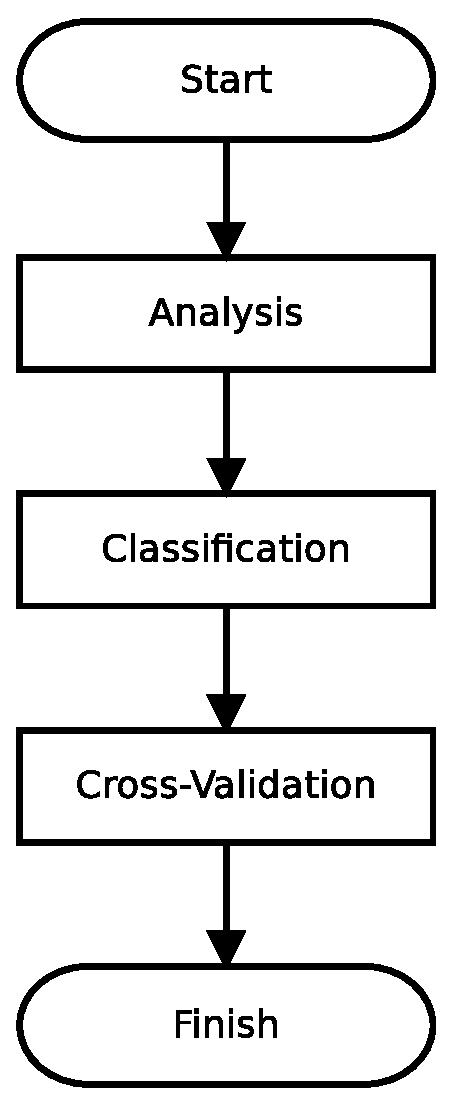
\includegraphics[width=\linewidth]{img/basic-arch}
\caption{Basic Overall Architecture}\label{fig:basic-arch}
\end{figure}

Building up from this it is apparent that to implement the analysis and classification steps that 
there is a need to implement the factory method design 
pattern\cite[p.~93-100]{Gamma1996Entwurfsmuster}. Reading from a data source should be a simple
matter of reading from a file, and cross validation has already been decided to use leave-one-out
cross validation.

Figure~\ref{fig:factory-arch} shows the design after adding in the factory methods.

\begin{figure}[h]
\centering
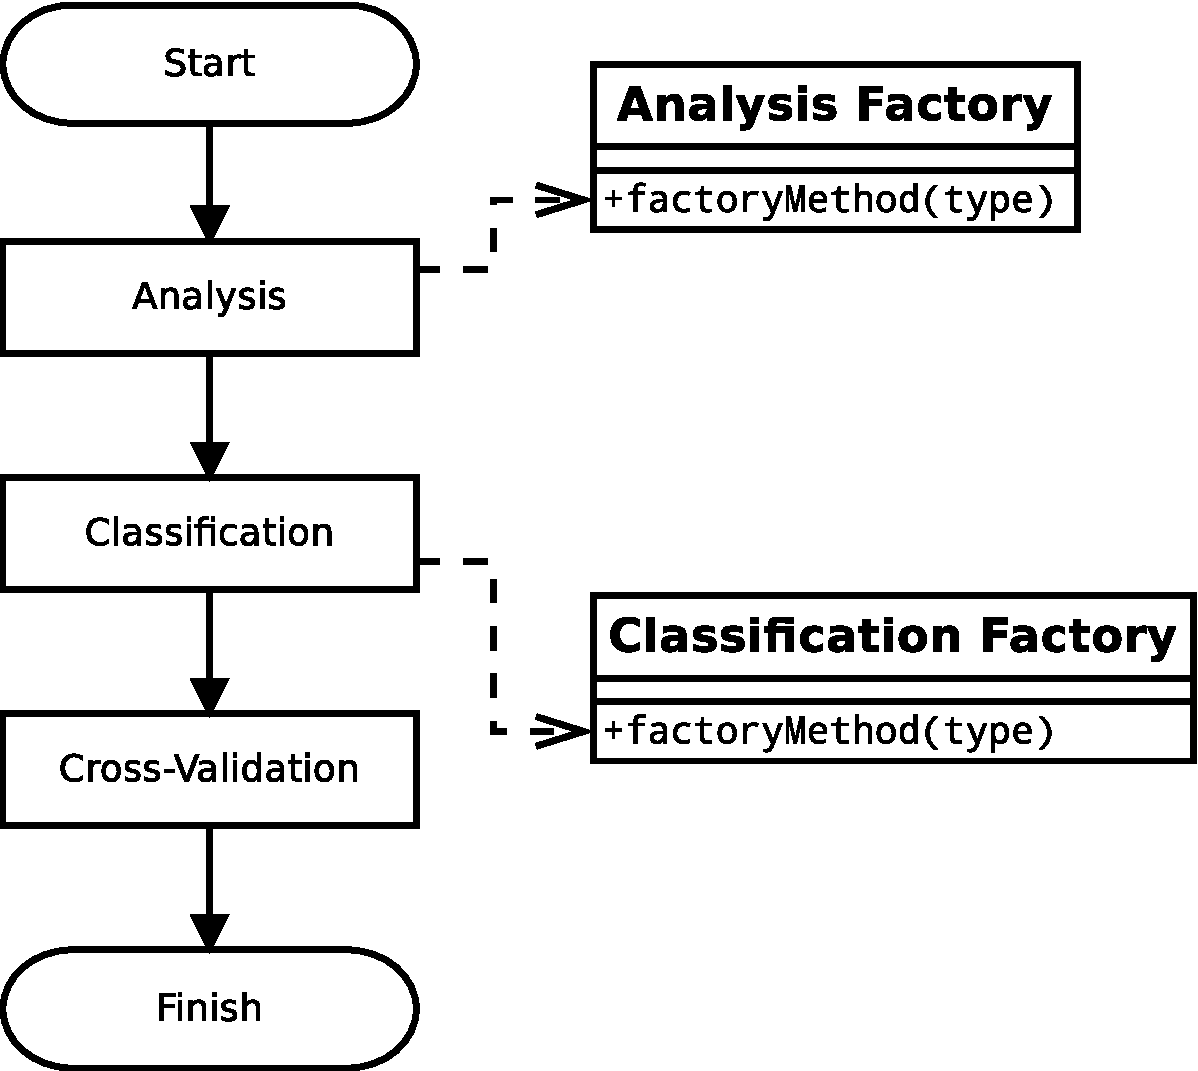
\includegraphics[width=\linewidth]{img/factory-arch}
\caption{Overall Architecture with Factory Methods}\label{fig:factory-arch}
\end{figure}

From this we then need the two top-level interfaces \verb+Analyser+ and \verb+Classifier+. The 
\verb+Analyser+ interface should have a single method which runs analysis on a painting and return
some form of object which represents the analysed data.

The \verb+Classifier+ class should have a method which takes a single painting and a set of
paintings, returning a year which is the classified year of the single painting based on the set
of paintings.

At this point it is also required that there is a class to store meta-data of a painting. 
Figure~\ref{fig:interfaces-arch} depicts the design after adding in these parts.

\begin{figure}[h]
\centering
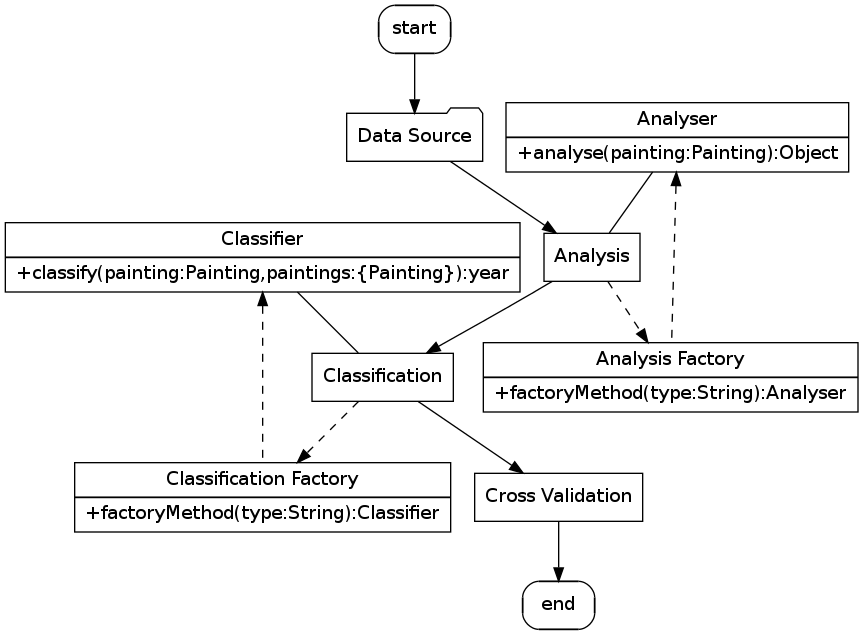
\includegraphics[width=\linewidth]{img/interfaces-arch}
\caption{Overall architecture with Interfaces for Analysers and Classifiers}\label{fig:interfaces-arch}
\end{figure}

\chapter{Implementation}

%The implementation should look at any issues you encountered as you tried to implement your design. During the work, you might have found that elements of your design were unnecessary or overly complex, perhaps third party libraries were available that simplified some of the functions that you intended to implement. If things were easier in some areas, then how did you adapt your project to take account of your findings?

%It is more likely that things were more complex than you first thought. In particular, were there any problems or difficulties that you found during implementation that you had to address? Did such problems simply delay you or were they more significant? Your implementation might well be described in the same chapter as Problems (see below).

\section{Research into Image Processing Libraries}\label{sec:cv-lib}

Due to the number of libraries out there and lack of experience in the area of computer vision and 
image processing, it was beneficial to research into some of the more popular libraries out there 
to get a feel for each library and image processing in general. This was done by creating a simple
application to perform Gaussian blur on an image, from this it was easy to gauge the use of the 
library and its documentation and could be extrapolated to see how difficult the library in 
question would be to use for more complex applications.

Table~\ref{tab:libraries-overview} shows an overview of all the libraries which were researched 
into.

\begin{table}[h]
\begin{tabular}{| c | c | c | c | c | c | c | c |}
								  \hline
\multirow{2}{*}{\textbf{Library}}	& \multicolumn{5}{|c|}{\textbf{Platform}}			& \multirow{2}{*}{\textbf{Language(s)}}	& \textbf{Example}	\\\cline{2-6}
					&  Windows	& Mac 		& Linux 	& Android	& iOS	&			&			\\\hline
\gls{opencv}					& \checkmark	& \checkmark	& \checkmark	& 		& 	& C, C++, Python	& Listing~\ref{lst:opencv}\\\hline
\gls{opencv} - cv2				& \checkmark	& \checkmark	& \checkmark	& \checkmark	& \checkmark & C, C++, Python, Java	& Listing~\ref{lst:cv2}\\\hline
FIJI					& \checkmark	& \checkmark	& \checkmark	& 		&	& Java			& Listing~\ref{lst:fiji}	\\\hline
IVT					& \checkmark	& \checkmark	& \checkmark	& 		&	& C++			& Listing~\ref{lst:ivt}	\\\hline
\end{tabular}
\caption{Comparison of image processing/computer vision libraries.}
\label{tab:libraries-overview}
\end{table}

\gls{opencv} appeared to be the most polished of all the libraries researched into, boasting a 
wide range of features with comprehensive documentation, especially for \gls{cv2}. 

\gls{fiji} has a good range of high-level features, especially through their GUI elements, however
for use as a library it was rather unwieldy and difficult to find the classes which performed 
simple functionality. Combined with equally bad documentation it was already unlikely to be used
but when, after fifteen minutes of struggling with the API images could only be blurred into a
grey-scale output, it was completely discounted.

It should be noted that most of the \gls{fiji} features weren't used at all and the actual code
seemed to just use ImageJ libraries.

\gls{ivt} was somewhat similar to \gls{fiji} in that it had a good range of high-level features, 
but was less impressive as a library. Despite following the example code it was difficult to 
compile against \gls{ivt}, despite using the makefiles provided in their own examples.

It was, therefore, an simple choice with only library being workable for this project. Not only
was \gls{opencv} the top choice from the above research, it is also one of the most prevalent
libraries for computer vision problems.

\gls{cv2} has been added to the above research as it shows how simplified many of the operations 
became after its discovery towards the end of the project.

\section{Basic Structure}

\subsection{Loading Data}
One of the more key parts to implement before all others in this project is the ability to load in
data from the initial spreadsheet. The first step of this was to convert it to a \gls{csv} 
file-type, which is easier to read programatically.

The initial spreadsheet was slightly different from the version depicted below, Lloyd was kind 
enough to update it so it was easier to handle digitally. In this version of the spreadsheet the
file names were much longer and were in sub-folders depending on their collection. Extra logic was
needed to locate the file (a simple matter of concatenating the collection to the file name as a
directory). The image files in the second version were just flat files which were better placed in
a separate data directory.

The move to the newer version was a good excuse to clean up some of the initial code to use better
Python programming practises; replacing messy loops with list comprehension where possible, using
\gls{kwargs} and dictionaries instead of having utility methods, etc.

From the original format show in table~\ref{tab:spreadsheet-format} the data was converted to the 
\gls{csv} format show in figure~\ref{fig:csv-spreadsheet}.

\begin{table}[h]
\resizebox{\textwidth}{!}{
\begin{tabular}{|c|c|c|c|c|c|c|c|c|c|c|c|c|} \hline
Filename & ID & Title & Catalogue entry BBC YP & Genre & Height & Width & Area & Materials & 
Collection & image width & image height & image height/image width \\ \hline
001.jpg & 1 & A Chapel in the Tyrol & 1950-1960 & Landscape & 40.7 & 29.8 & 1212.86 & oil on 
hardboard & NLW & 687 & 944 & 1.3741 \\ \hline
\end{tabular}
}
\caption{Layout of the Painting Data Spreadsheet}\label{tab:spreadsheet-format}
\end{table}

\begin{figure}[h]
\resizebox{\textwidth}{!}{
\texttt{001.jpg,1,A Chapel in the Tyrol,1950-1960,Landscape,40.7,29.8,1212.86,oil on hardboard,
NLW,687,944,1.3741}
}
\caption{Painting Data in CSV Format}\label{fig:csv-spreadsheet}
\end{figure}

This \gls{csv} file was then parsed using the Python 2.7 in-built \texttt{csv} module with 
relative ease. The example code (see listing~\ref{lst:csv_example_code}) helped to ensure correct
resource management as well as showing how the library parsed files.


\subsection{Top-Level Classes}
Being used to Java, the initial instinct was to set up interfaces for the majority of 
top-level classes (namely the \texttt{Analyser} and \texttt{Classifier} classes). However, 
Python does not have the concept of interfaces, so normal classes were used to represent these
instead. These classes acted as abstract stub classes and just held place-holder method definitions
which needed to be overridden in the concrete sub-classes. This was a slightly pointless exercise 
due to the duck typing, but was useful to depict the architecture in code. It also became more 
useful when these classes began to define a lot of the common methods.

A \texttt{Painting} class was also implemented and had a builder method to take an array (from the
\gls{csv} file) and create a new instance of it from this. Later this was changed to make use 
Python \gls{kwargs} instead to make it easier to both read and process, especially in the exemplar
work where mock objects were used.


\subsection{Command Line Interface}
As a research program with lots of different analysis and classification techniques the next step
in setting up the basic architecture was to create a set of command-line arguments which would
switch the functionality of the program. These arguments are depicted in table~\ref{tab:args}.

\begin{table}[h]
\centering
\begin{tabular}{|c|c|c|c|} \hline
Name             & Short Flag & Long Flag         & Description\\\hline
Analyser         & \verb+-a+  & \verb+--analyser  +& Switch the analysis technique\\
Machine Learning & \verb+-m+  & \verb+--ml        +& Switch the machine learning technique\\
Data             & \verb+-d+  & \verb+--csv       +& The data file to use\\
GUI              & \verb+-g+  & \verb+--gui       +& Switch the GUI visualisation\\
Binning          & \verb+-5+  & \verb+--bin-years +& Put paintings in 5 year bins\\
Export           & \verb+-e+  & \verb+--export    +& Export analysed data\\
Classify         & \verb+-c+  & \verb+--classify  +& Classify the specified image\\
\hline
\end{tabular}
\caption{Command Line Arguments}\label{tab:args}
\end{table}

The \texttt{argparse} library handles this nicely, the example code shown in 
listing~\ref{lst:argparse_example_code} shows the usage of this library.

These flags then hook into the factory methods to actually create the instances and return them to
the central point which then called them where required. A 
fa\c{c}ade\cite[p.185-194]{Gamma1996Design} was used to hold and call these instances, as well as
handling the calls to the factories.


\section{Colour Space Analysis}
Colour space analysis involves performing statistical analysis on different colour models 
(\gls{rgb}, \gls{hsv}, etc.). This gives a very simplistic view of the entire image.

\gls{opencv} offers a method to perform the average across the image, however with a
further look into the documentation there is also a method which performs both 
mean and standard deviation on an image.

The analysed data was just the tuple returned by this method. The distance measure
was defined to be the sum of all elements in the tuple (in the case of an \gls{rgb} colour model
the mean red, green and blue and the standard deviation of red, green and blue).

\subsection{Colour Models}
There are many colour models to consider with digital image processing. \Gls{rgb} is one of the
better know colour spaces as it is often how images are captured. It does have a problem in that
all three values can change when the brightness changes.

As one of the main principals of this project is that Williams' work darkened over time, it
should follow that \gls{rgb} may not be the best colour model to use.

To account for this it was decided to also use a \gls{hsv} colour model to compare and contrast to
\gls{rgb}.

\gls{opencv} handles colour spaces slightly oddly. Initially it uses a method to load the 
image, which uses an integer argument as a flag to define whether the image should be loaded in 
colour or grey-scale.

From this image you then can use a function to convert the colour model of an image, which 
uses an integer argument as a flag to define a number of different colour spaces.

Once converted, all methods act exactly the same as they would on a \gls{rgb} image.

\subsection{Colour Histograms}
Colour Histograms are a representation of the distribution of colour across an image; this makes
them very powerful for analysing the colour space of an image.

\gls{opencv} provides a number of methods for both calculating and operating upon colour histograms. 
Here the example code (figure~\ref{lst:opencv_histogram}) from the \gls{opencv} documentation was a
useful reference as some of the details of creating histograms in \gls{opencv} are not noted implicitly
in the python documentation.

The distance measure between colour histograms is also handled by \gls{opencv} using a compare histogram
method. Under the covers this uses a Chi Squared ($\chi^2$) (equation~\ref{eq:chi_squared}) method to
compare to histograms of equal dimensions.

\begin{equation}\label{eq:chi_squared}
\chi^2(H_1,H_2) =\sum_I{\frac{(H_1(I) - H_2(I))^2}{H_1(I)}}
\end{equation}

It should be noted that this method includes normalisation so any histograms passed into $\chi^2$
do not need to be, themselves, normalised.


\section{Texture Analysis}

\subsection{Edge Count}
The simplest technique to analyse texture is to apply an edge detection algorithm over the image
and produce a count of all the marked edges regardless of orientation.

The Canny edge detector\cite{Canny1986Computational} provided a good output for measuring this, 
operators like Sobel provided less useful results and thus provided a worse analysis technique.

From the generated image a histogram was produced with only 2 bins; one bin for the presence of an
edge, the other for the absence of an edge.

Open CV provides methods for applying the Canny edge detector to an image so this technique was 
simple to implement.

%TODO Image of the Canny'd image.

\subsection{Histograms of Orientation Gradients}
This technique is based on the \gls{hog} paper\cite{Dalal2005Histograms} and mirrors some of the
implementation in a simplified fashion.

The main crux of the method was to generate the exact orientation of a given point of an image,
apply this across the image and then bin the results into a histogram. The original paper then
focused on using this for human recognition and aimed to keep the time complexity down through
normalisation, applying it to this project only needed the generation of the histogram of exact
orientations.

Calculating the edge orientation involves passing a filter over an image which is used to find the
orientation of that gradient. 

There are many forms of filter which can be used to do this. The simplest of which discrete 
derivative masks (figure~\ref{fig:1x2-ddm}, figure~\ref{fig:1x3-ddm}, etc.), steerable filters 
are a more adjustable implementation of this. There are also more complex filters, like Gabor 
filters, which provide better flexibility and matching.

Using discrete derivative masks it is fairly simple to work out to orientation of a gradient 
mathematically. First pass a mask of the form $\left[\begin{smallmatrix}-1\\0\\1\end{smallmatrix}\right]$, followed
by one in the form $\left[\begin{smallmatrix}-1 & 0 & 1\end{smallmatrix}\right]$. These give 
$\frac{\delta f}{\delta x}$ and $\frac{\delta f}{\delta y}$ respectively.

A gradient direction function, shown in equation~\ref{eq:grad_dir}, can then be used on both these
values to work out the actual direction of the gradient.

\begin{equation} \label{eq:grad_dir}
\theta = {\rm atan2}\left( \frac{\delta f}{\delta x}, \frac{\delta f}{\delta y} \right)
\end{equation}

\subsubsection{Canning of Histogram of Orientated Gradient Results}\label{sec:hog-canning}
Working out the exact orientation of a gradient is a costly operation and it became useful to
\emph{can} (persist) the results to allow the technique to complete in a decent amount of time.
This change was made after the change to \gls{cv2} and was done using numpy methods for
simplicity. 

Rather than can the resulting histograms it was actually easier to can the output gradients as 
this allowed histograms with varying bin sizes to be used; this allows a comparison between 
steerable and Gabor filters to these histograms.

\subsection{Steerable Filters}
Another way of doing this is to change the orientation of the filter and bin the direction into 
certain cardinal directions; typically $0$, $\frac{\pi}{4}$, $\frac{\pi}{2}$ and $\frac{3\pi}{4}$
(from $\pi$ to $2\pi$ becomes a repeat of any of those directions, only in reverse and are, 
therefore, covered already).

To do this we can use steerable filters $S(\theta)$ (shown in figure~\ref{fig:steerable-filters}). 
With these we adjust the angle they are designed to match ($\theta$), which will then give the 
degree to which a gradient matches that angle. To complete the binning by orientation, this value 
will then have a threshold applied, then added to the bin if the value is above the threshold.

\begin{figure}[h]
$$
S\left(0\right) = 
\begin{bmatrix}
0 & 1 & 0 \\
0 & 1 & 0 \\
0 & 1 & 0
\end{bmatrix}
S\left(\frac{\pi}{4}\right) =
\begin{bmatrix}
0 & 0 & 1 \\
0 & 1 & 0 \\
1 & 0 & 0
\end{bmatrix}
S\left(\frac{\pi}{2}\right) = 
\begin{bmatrix}
0 & 0 & 0 \\
1 & 1 & 1 \\
0 & 0 & 0
\end{bmatrix}
S\left(\frac{3\pi}{4}\right) = 
\begin{bmatrix}
1 & 0 & 0 \\
0 & 1 & 0 \\
0 & 0 & 1
\end{bmatrix}
$$
\caption{Steerable Filters}
\label{fig:steerable-filters}
\end{figure}

These have the advantage of being far less complex to compute than edge orientation; the maths and
histogram creation on a floating point array are long running operations, to the point where
canning the results for edge orientation is desirable.

There is the obvious trade off that steerable filters can only work in four directions which
does affect the performance quite severely.

\subsection{Gabor Filters}
To increase the orientations matched from steerable filters without the need for increasingly 
large kernels, Gabor filters\cite{Daugman1985Uncertainty} were implemented. Gabor filters allow
for an almost-infinite range of orientations without affecting the size of the filter. Equation
\ref{eq:gabor} shows the mathematics used to generate a Gabor Filter.


\begin{align}\label{eq:gabor}
g(x, y; \lambda, \theta, \psi, \sigma, \gamma) &= \exp \left( -\frac{x'^2+\gamma^2y'^2}{2\sigma^2} \right) \cos \left( 2\pi \frac{x'}{\lambda} + \psi \right)
\intertext{where:}
x' &= x \cos \theta + y \sin \theta \nonumber \\
y' &= x \sin \theta + y \cos \theta \nonumber
\end{align}

As with steerable filters the results of the filter were passed into a histogram. Initially Gabor
filters were implemented with the same 4 orientations as steerable filters ($0$, $\frac{\pi}{4}$,
$\frac{\pi}{2}$ and $\frac{3\pi}{4}$), however this has two problems:

\begin{enumerate}
\item The variation in orientations is not being utilised and,
\item Divide by 0 errors from python.
\end{enumerate}

To solve both of these issues the way Gabor filters were initialised was changed by adding in a 
parameter which defined the number of orientations that instance of the Gabor filter would have,
the logic of which is defined in figure~\ref{fig:gabor-init}, note how the range is $1\dots b$, 
solving the divide by 0 issue as $\theta=0$ and $\theta=\pi$ will produce the same result (both
matching vertical lines best).

\begin{figure}[h]
\begin{algorithmic}
\Function{Gabor.init}{$b$} \Comment{$b$ is the number of orientations}
\For {$i \in 1\dots b$}
\State $\theta_i \gets \frac{i\pi}{b}$ \Comment{$\theta$ is the list of orientations to produce filters for}
\EndFor
\EndFunction
\end{algorithmic}
\caption[Psuedocode for Gabor Filter initialisation]{Psuedocode for Gabor Filter initialisation including number of orientations to produce 
filters for}\label{fig:gabor-init}
\end{figure}

The actual Gabor filters are then produced for all values in $\theta$ at runtime and applied to
the images in turn.

\section{Brush-Stroke Analysis}

Due to time constraints it was not viable to look at brush-stroke analysis, especially with the
shift of focus to exemplars after texture analysis.

It would have been nice to explore this area due to Williams' style, but a lack of high-resolution
images would have also made this a difficult area to get right.

There were several good ideas thought of for this area. One was to train a machine learning 
technique to recognise brush-strokes through the manual marking of strokes. This would have been a
very interesting method to try, especially being able to apply existing techniques to aid and
improve the classification of brush-strokes.

Other techniques involved passing filters over the image looking for the edges of brush-strokes
\cite{Berezhnoy2009Automatic}, then applying other operations to complete the stroke area. This
is a much simpler technique which will likely give bad results due to the low resolution and
non-uniform scaling of the images as it seems to be very dependant on the filter.

One final technique suggested by Li et al.\cite{Li2012Rhythmic} involves a combination of edge
analysis and clustering in colour space with a number of heuristics involving branching, 
stroke-width modelling and gap filling to refine the original brush-stroke estimates.

The difficulty that would be associated with this section of work is that existing techniques may
not be applicable to Williams' work due to his use of the palette knife. Whilst there are very
obviously clear strokes in his work, comparing these strokes to the likes of Van Gogh are unlikely
to pay off due to the \emph{blockier} strokes of the palette knife. Another reason this analysis
technique was side-lined in favour of exemplars.


\section{Ensemble Methods}
Ensemble methods are commonly used in statistical and machine learning to improve the performance,
the main concept of an ensemble method is to combine two or more models to produce better results
than would be gained from a single model.

Practically, ensemble methods just involve running all models in the ensemble, combining them into
one large histogram and then perform the normal distance measure on them. However, due to some 
problems with the \gls{cv2} histogram calculation method, it was a lot easier to flatten
(to collapse a multi-dimensional array into a one-dimensional array) the results from each 
technique have use this as the model.

This does affect the performance a little, but it is better than the other solution of adding 
resulting distance from each model together as the distances are not normalised. This was my 
initial solution to the problem and hugely affected the results as the distance returned from
statistical colour-space methods is a lot less than those returned from colour histograms and so
on.

Of course it would also be possible to normalise each distance measure of each technique, but this
would be difficult as the mean and variance of the distance for an analysis technique is not 
tracked. It may also cause problems when new examples are added (during validation, for example)
which affect both these values.

This method is commonly known as \gls{bagging}; where each model has a ``vote'' with equal weight.

One part I considered adding to this, but didn't have the time to complete, would be to weight the
vote of each technique (likely via a machine learning technique) in the ensemble so that the 
better performing techniques affect the results more.

Another method commonly used in machine learning is Boosting, where the model is built 
incrementally, with the focus being on examples which were mis-classified by the previous models.
This method does improve accuracy, but is known to over-fit the data set. 


\section{Classification and Validation}
With the results of analysis techniques there's also a need to be able to classify paintings based
on these results and also to validate the results of both so that different methods of analysis
and classification can be compared for performance.

\subsection{$k$-Nearest Neighbour}
The simplest method of classification is to work out which painting in the data set is closest in
feature space to the painting which needs to be classified and classify the year of this painting
with the year of the nearest painting.

This is effective a $k$-Nearest Neighbour with $k=1$, figure~\ref{fig:1nn} shows the psuedocode
for this algorithm

\begin{figure}[h]
\begin{algorithmic}
\Function{1-NN}{$p$, $data$}
\State $n = \operatorname*{arg\,min}_{d \in data}$ \Call{Distance}{$p, d$}
\State\Return $n_{year}$
\EndFunction
\end{algorithmic}
\caption{Psuedocode for 1-Nearest Neighbour}\label{fig:1nn}
\end{figure}

From 1-Nearest Neighbour it is a simple matter to change this to a $k$-Nearest Neighbour algorithm
as figure~\ref{fig:knn} shows.

\begin{figure}[h]
\begin{algorithmic}
\Function{k-NN}{$p$, $data$, $k$}
\ForAll {$k$}
\State $n = \operatorname*{arg\,min}_{d \in data}$ \Call{Distance}{$p, d$}
\State $a \gets a + n_{year}$
\State $data \gets data \setminus n$
\EndFor
\State \Return \Call{Average}{$a$}
\EndFunction
\end{algorithmic}
\caption{Psuedocode for $k$-Nearest Neighbour}\label{fig:knn}
\end{figure}

With this, the method of averaging the year can be any statistical method of taking the average
(mean, median or mode). Mean is the typical case for $k$-Nearest Neighbour as it is simple to
implement. Median is less common as it is slightly more complex to implement. Mode is more 
difficult to implement programmatically, especially given the sparseness of the data. 

$k$-Nearest Neighbour is good for this project as it makes no assumptions about the state of the
data, it only uses points in feature space to function. Initially, when feature space data wasn't
stored exclusively in histograms with was useful as it allowed different distance measure to be
applied without needing to change the classifier.


\subsection{Leave-One-Out Cross Validation}
To validate the classified years from $k$-Nearest Neighbour, this project uses Leave-one-out Cross
Validation; a technique which involves removing each point from the known data set, applying the
classification technique to this point against the remaining data set. This produces a list of
classified years against the actual years.

To measure the goodness of fit the Pearson's product-moment correlation coefficient was 
calculated on these orderings; this provides us with a performance measure of each classifier. 
It is also possible to test Pearson's R for statistical significance.

Pearson's correlation is perfect for this project; A perfect correlation of $1$ is achieved by
having the classified years exactly match the actual years.

Both of these are easy to implement - leave-one-out cross validation just involves iterating over
the entire list of known paintings, popping the current painting from the list and running the 
classifier on it, then pushing it back into the list at it's original position. Pearson's 
correlation is implemented by numpy with Pearson's R for statistical significance included
as a part of the method.

As a part of this matplotlib was used to plot this data graphically; as a scatter plot for
actual versus classified year and as a histogram for the number of years out the classifier was.

%TODO Scatter plot
%TODO histogram of years out


\subsection{Weka 3}
Weka is a collection of machine learning algorithms\cite{Hall2009WEKA}, used predominately for
data mining. Due to the number of machine learning techniques it provides it was interesting to
input data from the analysis techniques into Weka.

%TODO More on Weka


\subsubsection{Attribute-Relation File Format (ARFF)}
Part of inputting data into Weka is to produce \gls{arff} from the
analysis techniques. \gls{arff} is the main format supported by Weka, so it is one of the easiest ways
of importing the data into Weka.

A few libraries exist for \gls{arff} conversion in Python, however they all have their own quirks. 
liac-arff was one of the easiest to use, but doesn't support the date attribute. This isn't
a problem for our current project as we only use year which can easily be represented as an 
integer instead. I did intend to contribute a working patch for dates for the library, but it 
would have taken too much time out of the project to get it working correctly.

To be able to export in \gls{arff} file some translation from \gls{opencv} structures to raw data is 
needed. To begin with (whilst still not using \gls{cv2}) this was easiest done by exporting 
complex \gls{opencv} to a file using the functions provided by \gls{opencv}, then read back from
this file in for each painting.

To do this the Python operating system library was used to create a named temporary file, then to
pass the name of this file to \gls{opencv} (which only takes a file name and not a file descriptor
or any other form of pointer). 

The output from \gls{opencv} export methods is a \gls{yaml} - a human-readable data serialisation
format - which is well supported by Python. This data can then be read back in a non-\gls{opencv}
data structure and then re-exported using the \gls{arff} method described above.

The other option would be to find a parser which converts the \gls{yaml} format to an \gls{arff} 
one. However no such parser currently exists. Whilst this would be a nice tool to write and
contribute back to Python, the time it would take to do so would not outweigh the benefits.


\subsection{Exemplars}
Another method of classification is to incorporate expert knowledge within the framework. For each
year represented in the collection Dr Paul Joyner, of the National Library of Wales was asked to
choose the one painting which best represented Williams' work for that year. Dr. Joyner is a 
member of the Trustees of the Kyffin Williams Estate and he has written widely on Welsh Art and
Kyffin Williams.

These chosen paintings are considered to be connoisseurially or artistically selected exemplars
(\emph{artistic exemplars}, for short), which can be used as a representation of that particular
year.


\subsubsection{Nearest Exemplar Classification}
The most obvious use for artistic exemplars is to classify a given example using the nearest 
artistic exemplar, rather than other members of the data set, as depicted in 
figure~\ref{fig:nearest-exemplar}.

\begin{figure}[h]
\begin{algorithmic}
\Function{NearestExemplar}{$p$}
\State $n \gets \operatorname*{arg\,min}_{e \in exemplars}$ \Call{Distance}{$p$,$e$}
\State \Return $n_{year}$
\EndFunction
\end{algorithmic}
\caption{Psuedocode for Nearest Exemplar Classification}\label{fig:nearest-exemplar}
\end{figure}

To implement Nearest Exemplar Classification was a fairly easy task: a secondary spreadsheet was 
provided which contained all the necessary information of exemplar by year (see 
table~\ref{tab:exemplar-spreadsheet} for the full document).

The spreadsheet was arranged in the format described in table~\ref{tab:exemplar-layout}, from
there it was a simple matter of saving the spreadsheet as a \gls{csv} file and taking some of the
existing code for parsing \gls{csv} files. This caused a slight problem in that the parsed data
didn't have enough information to create a full \texttt{Painting} object, yet all the analysis
techniques worked from these objects.

\begin{table}[h]
\centering
\begin{tabular}{|c|c|c|c|c|} \hline
Filename & ID  & Title                      & Catalogue Entry & Year \\\hline
154.jpg  & 154 & Landscape at Llanaelhaearn & 1947            & 1947 \\\hline
\multicolumn{5}{|c|}{\textit{etc.}}\\\hline
\end{tabular}
\caption{Layout of the Exemplar Spreadsheet}\label{tab:exemplar-layout}
\end{table}

This was solved easily thanks to Python's dynamic typing. A simple class which implemented all the
necessary elements of \texttt{Painting} could be passed to the analysis techniques without any
complaints. With a statically typed language this would have been harder to complete, but there
would have been ways around using sub-classes and so on.

With the exemplars loaded and analysed, the program could continue as normal, until the
classification step.

The idea of Nearest Exemplar Classification is to classify the unknown example using the nearest
exemplar to that example in the feature space. This acts as a $k$-Nearest Neighbour with $k=1$ and
the space of neighbours only including the exemplars, rather than every other example. The 
psuedocode for this is shown in figure~\ref{fig:nec-psuedo}.

Initially this was implemented so that the examples that were exemplars were also classified, but
this is a pointless exercise which only skews the results. Additional logic to remove any exemplar
which matched the current example.

\begin{figure}[h]
\begin{algorithmic}
\Function{NearestExemplarClassification}{$p$}
\State $n \gets \operatorname*{arg\,min}_{e \in exemplars \setminus p}$ \Call{Distance}{$p$, $e$}
\State \Return $n_{year}$
\EndFunction
\end{algorithmic}
\caption[Psuedocode for Nearest Exemplar Classification with Added Logic]{Psuedocode for Nearest Exemplar Classification with Logic to Remove $p$ from $exemplars$}\label{fig:nec-psuedo}
\end{figure}

This proved to give slightly worse correlation per technique than $k$-Nearest Neighbour. This 
result is to be expected; for a start an artistically classified exemplar is unlikely to be the
same as a statistically classified exemplar (see section~\ref{sec:sce}). Also, with fewer examples
to classify against, any variance in the data set (of which there is a lot) will likely be 
magnified.

Lastly, a painting may be picked as an exemplar by an expert for different reasons than any
analysis technique that currently exists can give; emotional connections and knowledge of the
artists history can be very subjective and may not relate to anything put down in paint.


\subsection{Statistically Classified Exemplars}\label{sec:sce}

Another approach to exemplars is to work out a theoretical exemplar for a given period; the 
centroid of paintings within the given feature space for a single year, for example. 
Figure~\ref{fig:centroid} shows how a centroid is generated for three points in a 2D feature
space. However, for a high-dimension feature space this method needs to be simplified.

\begin{figure}[h]
\centering
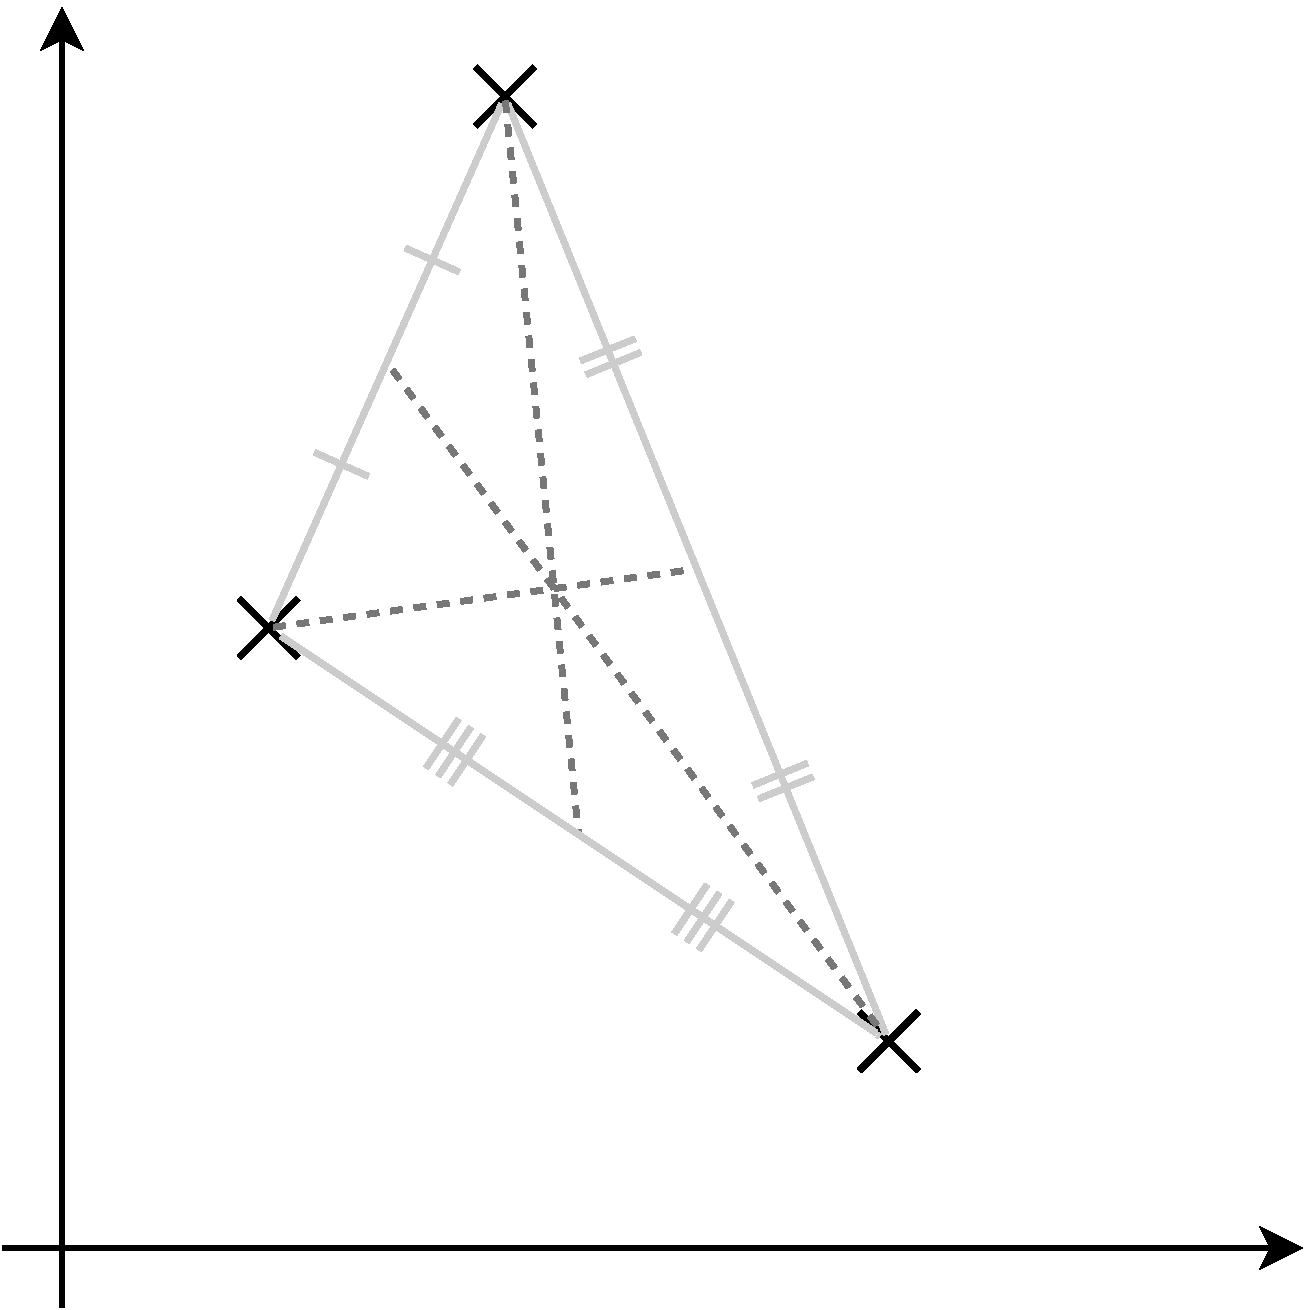
\includegraphics[width=0.5\textwidth]{img/centroid.pdf}
\caption{Centroid for three points in a 2 dimensional feature space}\label{fig:centroid}
\end{figure}

Equation~\ref{eq:sce} shows how the centroid ($C$) can be generated in a high-dimensional feature 
space (of $D$ dimensions), this works by taking the mean (equation~\ref{eq:mean}) of each feature 
in the set of paintings ($x_1, x_2,\dotsc,x_k$) for a single year, this will give the point in 
feature space that is most central. This is the same technique used to generate centroids in most 
clustering algorithms ($k$-Means Clustering, for example).

\begin{equation}
\label{eq:sce}
\forall_{d \in D}\;C_d = \frac{1}{k}\sum^{k}_{i=1}{x_{i_{d}}}
\end{equation}

%\begin{figure}[h]
%\begin{algorithmic}
%\Function{StatisticalClassifyExemplar}{$examples$}
%\ForAll{$example \in examples$}
%\ForAll{$feature \in example_{features}$}
%\State $average_{feature} \gets average_{feature} + example_{feature}$
%\EndFor
%\EndFor
%\ForAll{$feature \in average$}
%\State$average_{feature} \gets \frac{average_{feature}}{\Call{Length}{examples}}$
%\EndFor
%\State \Return $average$
%\EndFunction
%\end{algorithmic}
%\caption{Psuedocode for generating a Statistically Classified Exemplar}\label{fig:sce-psuedo}
%\end{figure}

This may become a long operation depending on how many dimensions the feature space has. A
technique like \gls{pca} may be useful to help cut down the number of dimensions needed that this
algorithm uses.

Initially, as I wasn't producing histogram results from analysis techniques, this was a little
complex to do; each analysis technique had to have its own method of generating the centroid and
returning the data for this centroid. The change to histogram results made everything a lot easier
and, combined with the mean method from numpy, which can handle the mean along 
different axes, rather than just over a flattened array. This is the perfect too for the job as
histograms are returned as numpy arrays and the data passed into the centroid method is now an 
array of these histograms. Calculating the mean across the first axis has the effect of 
calculating the centroid. Equation~\ref{eq:mean-matricies} shows this mathematically on 2D 
Matrices where $\bar{x}_n$ is the mathematical mean of $x$ along axis $n$.

\begin{align}
x=&\begin{bmatrix}
\begin{bmatrix}
1.0 & 1.0 & 0.0 \\
0.0 & 1.0 & 1.0 \\
0.0 & 0.4 & 0.0 \\
\end{bmatrix} & 
\begin{bmatrix}
0.0 & 1.0 & 0.0 \\
1.0 & 1.0 & 1.0 \\
0.6 & 0.0 & 1.0 \\
\end{bmatrix}
\end{bmatrix} \nonumber \\
\bar{x}_1 =& 
\begin{bmatrix}
0.5 & 1.0 & 0.0 \\
0.5 & 1.0 & 1.0 \\
0.3 & 0.2 & 0.5 \\
\end{bmatrix}
\label{eq:mean-matricies}
\end{align}

Whilst this is a useful theoretical exemplar, it doesn't fit with the idea of an artistic 
exemplar, it is quite possible that the art historians would be able to imagine a theoretical
painting which suits that year but they were limited to real paintings so it should follow that
the statistical exemplars can also be constrained in the same fashion.

This could be seen as a form of generalisation. Though this may affect the results for the worse
it may help prevent overfitting of the classification technique. It also shows which years are 
commonly chosen as exemplars correctly and incorrectly, this should give a vision of the 
difference between the artistic and statistic exemplars and where the artistic exemplars are the
outliers of that particular year.

To do this a 1-Nearest Neighbour algorithm is applied to the data for that year from the centroid,
this, of course, has the effect of picking the painting closest to the centroid, which is then
used as the exemplar for that year. The same technique used to classify using artistic exemplars
is then applied, only with these exemplars rather than the ones loaded from the exemplar file.

This then opened up the option to use inheritance to cut down on code repetition. The artistic
exemplar classifier could be extended by the centroid classifier, with a single method changed to
generate the centroids instead of reading them from a file. This, in turn, could then be extended
by the statistical exemplar classified (as described above) so that the 1-Nearest Neighbour
algorithm could be applied at the end of the generation of exemplars. Here the use of super calls
in Python gave me a little bit of trouble, listing~\ref{lst:py-super} shows one correct solution
to this\footnote{There are, of course, other correct methods, but the one listed is one of the 
better solutions}.

\begin{lstlisting}[language=python, breaklines=true, label=lst:py-super, 
caption={Super method calls in Python}, frame=single]
# Note Base has to extend 'object' for super calls to work
class Base(object):
    def call(self, params):
        # ...

class Sub(Base):
    def call(self, params):
        # Before Base.call
        super(self, Sub).call(params)
        # After Base.call
\end{lstlisting}


\subsection{cv2 and Histogram Results}
Whilst reading through the numpy and \gls{opencv} it turned out that, until this point, I had been
using a deprecated version of \gls{opencv}. \gls{cv2} is the new version of \gls{opencv} for 
python, which provides bindings for \gls{opencv} 2.4 and uses numpy arrays and multi-dimensional 
arrays to represent all data types rather than in-built data structures.

This makes everything a lot easier to work with as all numpy arrays (with the correct data type)
can be passed into the \gls{cv2} methods.


\section{Filtering}
One area that was experimented with was the ability to filter paintings by certain pieces of 
metadata for that painting. Typically with would allow the filtering of just a single type of
painting (e.g. filtering out any painting which isn't a landscape to remove potential outliers).

Unfortunately, with most techniques this produces worst correlation than not filtering by type,
this may be due to the limited size of the data set and purely by removing the non-landscape 
paintings leaves such a gap in the years that $k$-Nearest Neighbour cannot classify the painting
correctly.

A potential way of helping with this (and effectively filtering the data in a slightly different
fashion) is to round the year ($y$) of a painting to the nearest 5 years ($y_{_{5}}$). The maths 
to do this is shown in equation~\ref{5-years}. 

\begin{equation}\label{5-years}
y_{_{5}} = 5\left\lfloor\frac{y}{5} \right\rfloor
\end{equation}

This does improve the correlation by a little as it helps to counteract the sparseness of the data
in the data set. Whilst the improvements in correlation are nice, the information lost by rounding
is not really gained back by this increase in correlation.

\chapter{Testing}

%Detailed descriptions of every test case are definitely not what is required here. What is important is to show that you adopted a sensible strategy that was, in principle, capable of testing the system adequately even if you did not have the time to test the system fully.

%Have you tested your system on 'real users'? For example, if your system is supposed to solve a problem for a business, then it would be appropriate to present your approach to involve the users in the testing process and to record the results that you obtained. Depending on the level of detail, it is likely that you would put any detailed results in an appendix.

This chapter details the approach to testing and how validation was performed cross-validation was
performed to evaluate different analysis and classification techniques.

\section{Overall Approach to Testing}
As this is a research-based project, it is difficult to perform any for of unit, functional or 
requirements testing. Most testing is based on validating the results of analysis and 
classification techniques.

There is, however, a sense in which the validation of analysis techniques is a form of testing,
higher correlations would suggest that a given analysis technique is both implemented properly and
that it represents the data well.

There is also a sense in which testing that a technique does what it says it will is both 
difficult and somewhat unnecessary. One would expect to see the correlation increase as more
complex analysis techniques are implemented so if a recently implemented technique gives a lower
correlation that a previous technique then this might be considered as a failing test.

If the correlation is improved by the analysis then, even if the technique isn't working 
completely as advertised, it is still doing something right. It was common for the analysis to be
``tinkered'' with to try and improve the performance of the analysis so commonly any errors were
picked up at this point.

All analysis techniques were performed across two machines and typically acted similarly. The only
discrepancies noticed was on techniques which heavily relied on floating point numbers; usually a
few of the correlations were out by a proportionally tiny amount. This is believed to be because 
one system has a 32-bit operating system and the other a 64-bit.


\section{Validation}
Cross-validation is a statistical concept used to assess how the results of statistical analysis
generalise to an independent data set. Cross-validation is typically applied to machine learning
classifiers to test if a technique is overfitting the data; that is how specific the technique is
to the original data set and how it can cope with new examples. For example, a rote learner cannot
classify any unseen examples as the classification is performed based solely on the training set.

As the overall goal is to be able to classify any Williams painting it is important that the 
program is able to handle new examples, not just those for which the year is known.

There are many forms for calculating cross-validation, usually involving taking sub-samples of the
original data set and removing them from the training set to create a validation set.

$k$-fold cross-validation is a common method for performing this. It involves splitting the data
set into $k$ sections or \emph{fold}. Each fold is removed from the data set, the classifier is
trained on the remaining data, then the fold is classified using the trained data. 

The other common form of cross-validation is to take random sub-samples from the data set and are
removed from the training set and then classified using it. This process is performed repeatedly
until a good number of samples has been taken. This has advantages and disadvantages over $k$-fold
cross-validation, it has the problem that not all data points are considered during validation,
but doesn't depend on the size of the data set.


\subsection{Leave-One-Out Cross-Validation}
Leave-one-out cross-validation is a form of $k$-fold cross-validation in which the number of folds
is equal to the size of the data set. This leads to the behaviour of leaving a single data point
each time and classifying it against the rest of the data set. Because data sets in machine 
learning are typically very large this usually isn't an option due to time complexity.

However, because of the use of $k$-Nearest Neighbour-based classifiers (which need no re-training 
when data points are added or removed) and a small number of known data points, it is the best 
method of cross-validation for this project.

Leave-one-out cross-validation provides us with a classified year for each data point and, because
we only use data points with known years, we can then work out the correlation between actual and
classified years to get a value of performance.

To produce this value Pearson's product-moment correlation was used (equation~\ref{eq:pearsons})
the best techniques would produce a correlation value closer to $1$ than other techniques. Another
part of Pearson's is that it is easy to generate statistical significance (the p-value). This
describes the extent to which the observations could appear by chance in a given single null
hypothesis.

The results of the correlation between actual and classified year is defined to be $r$ 
(formally: $r=\rho_{classified, actual}$). The p-value is defined to be $P(r)$. The ultimate goal 
being to maximise $r$ whilst minimising $P(r)$.

Of course, an exact correlation of $r=1$ would be unrealistic to achieve, especially for such a 
humanities-based project. A good technique might reach correlations of $r \ge 0.5$ and a great
technique might reach correlations of $r \ge 0.75$.


%\subsection{Validation using Weka}


\chapter{Results}

The section shows the results from running the research on the dataset. These results focus on 
correlation coefficients and the differences between artistic and statistic exemplars.

\section{Correlation Coefficient Results}
One parameter for our classifier is the choice of $k$ for $k$-Nearest Neighbour. Simply setting 
$k=1$ has the effect of assigning the year of the nearest painting in feature space to the current
test painting, whilst setting $k=102$ has the effect of giving the painting the mean year of the 
entire data set. Obvious, a point between the two is likely to be the best. 

\begin{figure}[h]
\centering
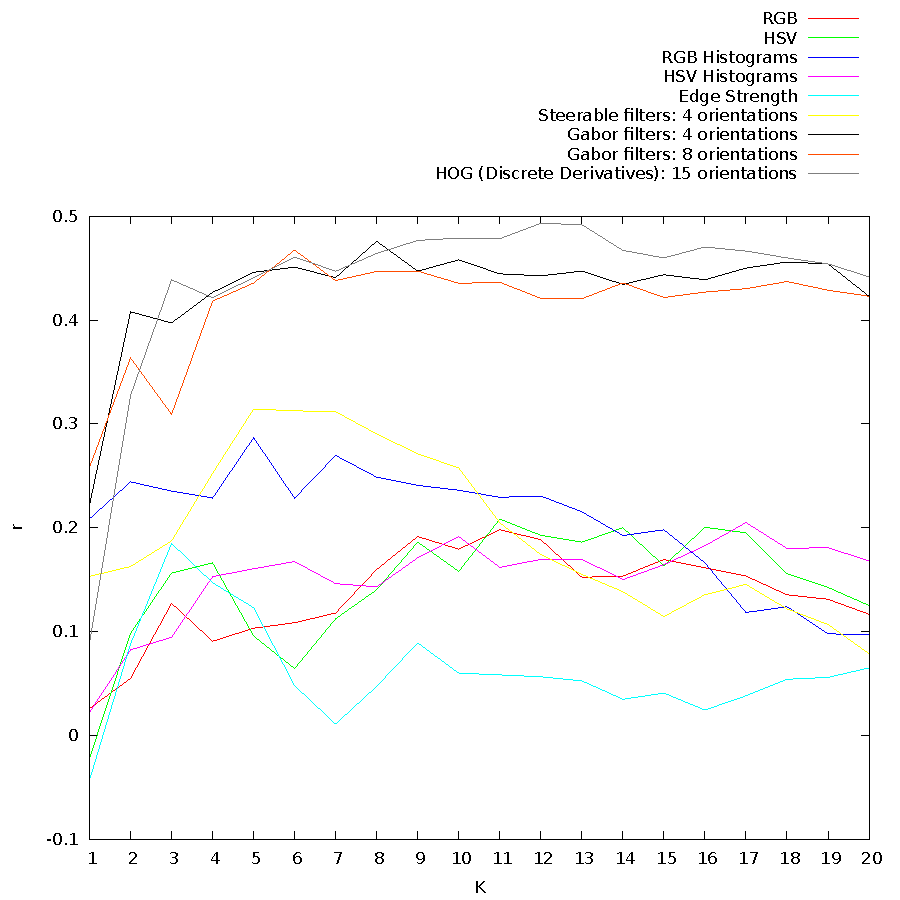
\includegraphics[width=0.9\textwidth]{../../isispa-paper/results/mean}
\caption{Correlation Coefficients $r$ against $k$ values for $k$-Nearest Neighbour}\label{fig:r-graph}
\end{figure}

From Figure~\ref{fig:r-graph} it is apparent that for many of the features spaces we have that the 
optimum value of $k$ is around 7 or 8. Table~\ref{tab:r-results} shows the actual results for each 
feature space for a $k$ of 7, where $r$ is the correlation coefficient given by Pearson's, 
$P(r)$ is the p-value significance of $r$.

$C(n)$ is the percentage of paintings correctly classified within $n$ years of the actual year 
(where $E(X)-n \le X \le E(X)+n$).

\begin{table}[h]
\centering
\begin{tabular}{|l|c|c|c|}\hline
Technique     					& $r$    & $P(r)$ & $C(15)$ \\ \hline
Edge Strength 					& 0.0107 & 0.910  & 60\%    \\
HSV 						& 0.112	 & 0.237  & 64\%    \\
RGB 						& 0.118  & 0.214  & 63\%    \\
HSV Histograms					& 0.146	 & 0.123  & 64\%    \\
RGB Histograms					& 0.270	 & 0.004  & 62\%    \\
HOG (Discrete Derivatives): 4 orientations 	& 0.307	 & 0.001  & 65\%    \\
Steerable filters: 4 orientations 		& 0.312	 & 0.001  & 68\%    \\
HOG (Discrete Derivatives): 8 orientations 	& 0.346	 & \textless0.001 & 65\% \\
HOG (Discrete Derivatives): 16 orientations 	& 0.367	 & \textless0.001 & 64\% \\
Gabor filters: 16 orientations			& 0.370  & \textless0.001 & 67\% \\
Gabor filters: 8 orientations			& 0.438	 & \textless0.001 & 70\% \\
Gabor filters: 4 orientations			& 0.441	 & \textless0.001 & 71\% \\
\hline
\end{tabular}
\caption{Correlation Coefficients, ordered by strength for $k=7$}\label{tab:r-results}
\end{table}


\newpage
\section{Ensemble Results}
Using ensemble methods can both improve and weaken the correlation coefficients depending on the
techniques used. The inclusion of colour histogram analysis and HSV colour-space statistical
analysis typically weakens the results, whilst combining \gls{hog} and Gabor filters typically 
improves the correlation coefficients beyond each technique individually. 
Table~\ref{tab:ensemble-results} shows some examples of this.

This does show that ensemble methods can help to improve the strength of analysis techniques, as
expected.

\begin{table}[h]
\centering
\begin{tabular}{|l|c|c|}\hline
Method	& $r$	& $P(r)$ \\ \hline
RGB 						& 0.118  & 0.214 \\
Ensemble RGB Histogram and HOG (16)		& 0.256 & 0.006 \\
RGB Histograms					& 0.269 & 0.004 \\
HOG (Discrete Derivatives): 16 orientations	& 0.367 & \textless0.001 \\
Ensemble RGB and HOG (16)			& 0.372 & \textless0.001 \\
Gabor filters: 4 orientations			& 0.441 & \textless0.001 \\
Ensemble RGB and Gabor (4)			& 0.443	& \textless0.001 \\
Ensemble RGB, Gabor (4) and HOG (16)		& 0.464	& \textless0.001 \\
\hline
\end{tabular}
\caption[Correlation Coefficients comparing individual and ensemble methods]{Correlation Coefficients comparing individual and ensemble methods. Note how the 
combination of RGB Histograms and \gls{hog} has decreased performance, whilst the combination of
\gls{hog} and Gabor filters has improved performance.}\label{tab:ensemble-results}
\end{table}

\newpage
\section{Exemplar Results}
The intuition -- that using artistically chosen exemplars could help to exploit knowledge about 
the way the paintings change over time -- turned out to be incorrect; results for Gabor filters 
with 4 orientations (the best performing method in our previous experiment) are shown in 
Table~\ref{artistic_exemplars}.  Results for the other feature spaces show a similar pattern, the 
same distance measure ($\chi^2$) has been used throughout. 

\begin{table}[h]
\centering
\begin{tabular}{|p{3.5cm}|c|c|c|}
\hline
Technique     & $r$ & $P(r)$ & $C(15)$ \\ \hline
%K=7
Artistic Exemplars	& 0.328	& \textless0.001 & 57\%\\
Statistical Exemplars	& 0.383	& \textless0.001 & 61\%\\
Centroid		& 0.403	& \textless0.001 & 64\%\\
\hline
\end{tabular}
\vspace{0.5em}
\caption{Correlation coefficients, ordered by strength, for Exemplars
\label{artistic_exemplars}}
\end{table}

These exemplars give an interesting insight into the feature space. The paintings shown in 
Figures~\ref{early_example} and~\ref{late_example} are both artistic exemplars, however the 
earlier painting ``\emph{Snowdon, the Traeth and the Frightened Horse}'', from 1948, is far from 
the feature space centroid for that year, whereas the later painting is very close to the feature 
space centroid for 1985. A visualisation of artistic exemplars and their corresponding statistical
representations is given in Figure~\ref{art_ex_stat_ex}. From this you can see that artistic 
information does not necessarily correspond well to the feature space(s) we use. Note that whilst 
Figure~\ref{art_ex_stat_ex} uses the feature space defined by Gabor filters with 4 orientations, 
our best performing: the pattern is similar for all other feature spaces.

\begin{figure}[h]
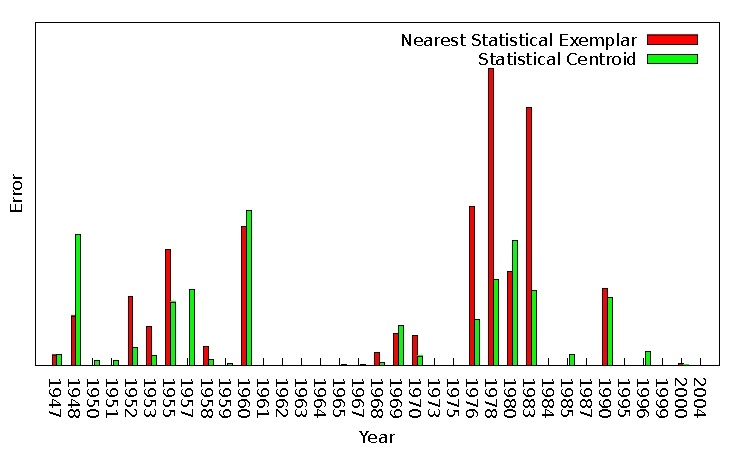
\includegraphics[width=\linewidth]{img/exemplar.pdf}
\caption[Distance in feature space from artistic to statistic exemplars]{Distance in feature space from artistic to statistic exemplars (red); distance from 
artistic exemplar to centroid (green). Lower values indicate that the artistic exemplar is near to
the mean painting for a particular year, higher values that an artistic exemplar painting is an 
outlier for this particular feature space\label{art_ex_stat_ex}}
\end{figure}

\chapter{Evaluation}

The chapter reflects back on the project to critically evaluate the main choices made. The three
main areas which this focuses on are the identification of requirements, the design decisions that
were made and the use of third party tools and libraries.

%Examiners expect to find in your dissertation a section addressing such questions as:

%\begin{itemize}
%   \item Were the requirements correctly identified? 
%   \item Were the design decisions correct?
%   \item Could a more suitable set of tools have been chosen?
%   \item How well did the software meet the needs of those who were expecting to use it?
%   \item How well were any other project aims achieved?
%   \item If you were starting again, what would you do differently?
%\end{itemize}

%Such material is regarded as the most important part of the dissertation; it should demonstrate that you are capable not only of carrying out a piece of work but also of thinking critically about how you did it and how you might have done it better. This is seen as an important part of an honours degree. You are expected to realise in which ways it falls short of perfection and of things that you did wrong.

%Sadly, the critical evaluation is the weakest aspect of most project dissertations. Because of its importance, some examples are provided on the project website.

\section{Evaluation of Requirements}
Due to this being a research project, the requirements were not well defined other than the end 
result of being able to classify paintings. Other requirements were added during meetings as new
problem areas were encountered but were never formally defined. This would have been a problem if 
the methodology used wasn't able to keep up with changing requirements.

Most of the aims that were defined to begin with were accomplished; in fact all but brush-stroke 
analysis were completed effectively. However, on further investigation the completion of 
brush-stroke analysis was not feasible for this project, the area is rather large and complex.
Also, with various time constraints, it turned out that exemplars were a more revealing, less 
time-consuming area of investigation.


\section{Evaluation of Design}
The initial design evolved very little over the course of the project, the main changes made were
to actually make use of inheritance to cut down on code-reuse. The design actively encouraged
this as it was set up to allow this activity.

The design wasn't perfect: until most of the way through the project, objects in parameters were 
manipulated to have properties set during the operation, instead of using return values from 
functions. Eventually this began to cause problems and was changed to correctly use return values
instead. Listing~\ref{lst:param-vs-ret} shows the changes made.

\begin{lstlisting}[caption={Using return values instead of manipulating parameters},
label=lst:param-vs-ret,
breaklines=true,
language=python,
frame=single]
# Manipulating parameters
def analyse(self, painting):
    img = imread(painting.file_path)
    painting.data = # specific analysis on img

# Using return correctly
def analyse(self, painting):
    img = imread(painting.file_path)
    return # specific analysis on img
\end{lstlisting}

Though this seems like a trivial change, it does affect how the code is called, especially in the
exemplar classification where affecting the painting data is not wanted.


\section{Evaluation of Tools}
This section is broken down into the evaluation of the choice of programming language and the 
image processing library used.

\subsection{Programming Language}
Python is a dynamic programming language which offers clear, reliable syntax; object orientation
including multiple inheritance; full modularity; exception-based error handling; and a good range
of dynamic data types.

Python was a good choice of programming language; it's dynamically typed nature allows a lot fewer
restrictions and though on the initial design, fitting well with the choice of methodology. 

Python was also very useful for built-in features like list comprehension (see 
listing~\ref{lst:python-list-comp} for an example), keeping the amount of code needed to build 
list- and dictionary- based elements down to a minimum. As well as other built-in operations on 
these data types, for example\texttt{zip} on two arrays to help graph results.

\begin{lstlisting}[language=python,
caption={Example of List Comprehension in Python},
label=lst:python-list-comp]
year = [painting.year for painting in self.paintings 
        if is_absolute(painting.year)]
\end{lstlisting}

Python also boasts a good number of libraries by default; libraries like the \gls{csv} parsing 
library used to read in data. These libraries provide a lot of extended functionality to the 
language. There is also the \gls{pypi} which allows the easy installation of 
additional packages.

A lack of experience in Python was a problem to begin with at first and a lot of the earlier code 
didn't utilise a lot of the useful features Python provides. However, after spending time 
contributing to an open source project, also written in Python, these skills quickly developed 
through feedback from commits and being able to read source code.

Java was a commonly suggested language, in part due to the wealth of experience there is within
the department. However, on investigation into image processing libraries, it was found that most
of these libraries were either difficult to work with or were not as complete as other available
options.

A recent beta version of \gls{opencv} 2.4.4 provides support for the Java programming language
for desktop users. However, this is vastly more complex to include as part of a project, requiring
additional tools like the Apache Ant build system. The use of a beta library would have also run the 
risk of running into bugs in the software and relying on the project to fix them. Due to constrained time it was the right decision not to
use \gls{opencv} with Java.

Java is also very constrained in the nature of typing and lacks a lot of the mathematical features
Python offers (list comprehension, lambda functions, etc.), which helps keep the code-base clean.
This combined with the verbose nature of Java would have increased the size of the project to
be less manageable.

Newer \gls{jvm} based languages, Scala for example, could have helped with this problem. But most
of the advantages gained by choosing Java as a language - especially knowledge - would have been
lost in doing so. These languages also still lack the mathematical features of Python.

As \gls{opencv} is natively written in C++, it might have made sense to use either C or C++ to write 
this project in, and both were strongly considered at the start of the project.

C lacks native object-orientation\footnote{Using structures and functions points it can mimic the 
behaviour to a certain extent, but still lacks inheritance} and is generally difficult to write 
``correctly''. Other issues like cross-platform support were also factors in the choice against C.

C++ has similar problems to C, though it does have more advanced features, including 
object-orientation, which do make it easier to work with. It can still be difficult to produce 
programs without problems. Both C and C++ have a decent set of compilers, from the standard 
\gls{gcc}, which provide very basic error helping features, to LLVM based compilers like clang which 
ease the process of finding bugs.

It was decided that, if the project ever managed to produce anything worthy of making into a
library, it would be ported to C++ and investigation would be made into contributing it back into
\gls{opencv}. This would have likely been related to the brush-stroke section of work in the project. 
The only other reason for using C++ or C over Python for this project, is if the processing needed
to be completed within a short period of time. As this is a research project it matters very 
little how fast each technique completes in\footnote{And, if a technique does take too long there 
are solutions to this problem through the canning of results, as was performed on \gls{hog} 
analysis (see Section~\ref{sec:hog-canning})}.

Newer, more popular languages like Ruby, don't have the support for image processing libraries and
the language features of Ruby don't particularly beat Python's. Many other languages suffer the
same flaws of not having good support for image processing libraries.

Python is not without its flaws, the lack of strictness, especially before running code, does mean
a lot of errors are encountered at runtime. This is a disadvantage of the dynamically typed and
interpreted nature of the language. Statically typed languages are a lot easier to pick up on
typing errors, whilst Python takes a step further than this and uses what is commonly known as duck
typing: ``If it looks like a duck and quacks like a duck, it must be a duck.''\cite{2013Glossary},
this means there's no direct need for the inheritance hierarchy. 

Not having a compiler to lean on for picking up syntax errors before runtime is another
disadvantage which Python suffers from. However, Python is generally quick enough to run that 
hitting these errors at runtime isn't a huge issue. There are also tools available to help pick up
on these errors. PyLint was used during the project to find syntax errors and clean up code to
typical Python standards. This was useful as most of the code was difficult to test cleanly so
runtime errors could be fairly common. The interpreter also has some checking for invalid syntax 
before runtime so it was useful to lean on that on occasion.

If the author were to take on this project again, Python still would have been the choice of 
language as the strengths detailed above far outweigh any of the weakness of the language.

\subsubsection{Dependency Management}
setuptools is a Python package designed to allow the easy downloading, building, 
installation, upgrading and uninstallation of Python packages from \gls{pypi}. It can be used to
manage the dependencies of a Python project through the use of a set-up file specifying the 
packages required for a project to run. On build of a project, all required packages will be 
downloaded and installed, along with any packages they in turn require.

Again this is a bonus of using Python. Java has very bad dependency management, the only tool
which is widely used to do this is Apache Maven, and is not widely adopted, therefore it is not all
that useful. \Gls{osgi} is another technology which makes managing dependencies easier, but in 
itself doesn't handle the download and installation of packages.

Languages like C and C++ tend to use packages through the operating system or user-based 
compilation. This can lead to a lot of dependency issues if the user is not well versed in the
installation of libraries from source. This is especially an issue on less common packages which are not provided
through a package manager\footnote{Or on Windows, which has no standardised package manager}.

Newer languages, again using Ruby as an example, do have better dependency management and tend to
be more tied to the language itself, rather than being a tool like setuptools. There aren't
many advantages to this as \gls{pypi} is widely known.


\subsection{Image Processing/Computer Vision Libraries}
There are numerous image processing and/or computer vision libraries available for use, each with
their own flavours and supported programming languages. \gls{opencv} was the eventual choice after a lot
of research into these libraries (as discussed in Section~\ref{sec:cv-lib}). \gls{opencv} is one
of the leading computer vision libraries freely available (released under the BSD License) and 
boasts an impressive number of methods. It has the benefit of being highly optimised and 
cross-platform.

In comparison to most other computer vision libraries \gls{opencv} feels well thought out and 
polished; with good, well written, documentation for all interfaces (C, C++ and Python). Some of
the Python documentation was a little difficult to use before discovering \gls{cv2}, but this was 
partly because it was no longer being maintained.

Other libraries, notably \gls{fiji}, lacked comprehensive, well laid out documentation. Method 
calls were either not obviously named or buried in so many namespaces that it was impossible to
find the correct call without documentation.


\subsubsection{OpenCV cv2}
Knowing about \gls{cv2} from the start would have been a useful piece of information, the
updates to the library made it a lot easier to use. For example; calling the calculate histogram
method in \gls{opencv} is shown in Listings~\ref{lst:cv1-hist}, whilst the same operation in 
\gls{cv2} is shown in Listings~\ref{lst:cv2-hist}. This is evidently a lot easier to call
and work with.



\begin{lstlisting}[language=python, caption={Creating a Histogram in OpenCV}, label=lst:cv1-hist, 
breaklines=true, frame=single]
import cv

image = cv.LoadImageM("file.png")

planes = [cv.CreateMat(image.rows, image.cols, cv.CV_8UC1) for i in xrange(3)]
planes = planes + [None]

cv.Split(image, planes)

hist = cv.CreateHist([255,255,255], cv.CV_HIST_ARRAY, [[0,255],[0,255],[0,255]], 1)
cv.CalcHist([cv.GetImage(i) for i in planes], hist)
\end{lstlisting}


\begin{lstlisting}[language=python, caption={Creating a Histogram in OpenCV cv2},
label=lst:cv2-hist, breaklines=true, frame=single]
import cv2

image = cv2.imread("file.png")
hist = cv2.calcHist([plane for plane in cv2.split(image)], [0], None, [255,255,255], [0,255,0,255,0,255])
\end{lstlisting}

Another advantage \gls{cv2} has is its tight integration with numpy - a numeric library for Python
and part of the scipy library. This integration allows many more complex operations to be 
performed on analysis results; operations which \gls{opencv} does not provide or provides in ways
only specific to image processing. A notable example of this is being able to take the mean along
an axis to generate the centroid in statistical exemplar classification.

numpy is also useful for non-image processing use; many complex mathematical functions are 
pre-defined. These are useful for generating the statistical results for a given set of analysis
and classification techniques, after leave-one-out cross validation is performed. The main use was
for Pearson's product-moment correlation coefficient and p-value significance.

Other libraries exist for these functions, but could not reasonably be considered due to the 
integration with \gls{cv2}.

% add any additional chapters here

\setemptyheader
\addcontentsline{toc}{chapter}{Appendices}
\chapter*{Appendices}
\pagebreak

% start the appendix - sets up different numbering
\fancypagestyle{plain}{%
%\fancyhf{} % clear all header and footer fields
\fancyhead[L]{\textsl{Appendix\ \thechapter}}
\fancyhead[R]{\textsl{\leftmark}}}

\appendix
\fancyhead[L]{\textsl{Appendix\ \thechapter}}
\fancyhead[R]{\textsl{\leftmark}}
\fancyhead[C]{}
\fancyfoot[C]{\thepage}
\renewcommand{\headrulewidth}{0.4pt}
\renewcommand{\chaptermark}[1]{\markboth{#1}{}}

\fancyhead[L]{\textsl{Appendix\ \thechapter}}
\fancyhead[R]{\textsl{\leftmark}}
\fancyfoot[C]{{\thepage} of \pageref{LastPage}}

% include any appendices here
\chapter{3\textsuperscript{rd} Party Libraries and Tools}


\section{Python 2.7}

\subsection{setuptools}
\url{http://pypi.python.org/pypi/setuptools}

\subsection{scipy}
\url{http://www.scipy.org/}\cite{EricJonesandTravisOliphantandPearuPetersonandothers2001SciPy}

\subsection{numpy}
\url{http://www.numpy.org/}\cite{EricJonesandTravisOliphantandPearuPetersonandothers2001SciPy}

\subsection{matplotlib}
\url{http://matplotlib.org/}

\subsection{liac-arff}
\url{https://github.com/renatopp/liac-arff}


\section{OpenCV}
\url{http://opencv.org/}\cite{opencv_library}

\subsection{OpenCV Python}
\url{http://opencv.willowgarage.com/wiki/PythonInterface}\cite{opencv_library}


\section{Weka 3}
\url{http://www.cs.waikato.ac.nz/ml/weka/}\cite{Hall2009WEKA}


\section{git}

\subsection{github}





\fancypagestyle{plain}{%
   \fancyhead{} %[C]{Annotated Bibliography}
   \fancyfoot[C]{{\thepage} of \pageref{LastPage}} % except the center
   \renewcommand{\headrulewidth}{0pt}
   \renewcommand{\footrulewidth}{0pt}
}

\setemptyheader

\nocite{*} % include everything from the bibliography, irrespective of whether it has been referenced.

% the following line is included so that the bibliography is also shown in the table of contents. There is the possibility that this is added to the previous page for the bibliography. To address this, a newline is added so that it appears on the first page for the bibliography. 
\addcontentsline{toc}{chapter}{Annotated Bibliography} % Adds References to contents page

%
% example of including an annotated bibliography. The current style is an author date one. If you want to change, comment out the line and uncomment the subsequent line. You should also modify the packages included at the top (see the notes earlier in the file) and then trash your aux files and re-run. 
\bibliographystyle{authordate2annot}
%\bibliographystyle{IEEEannot}
\renewcommand{\bibname}{Annotated Bibliography} 
\bibliography{References/references} % References file


\end{document}
